\documentclass[a3, landscape]{a0poster}
\usepackage{graphicx,lipsum}
\usepackage[paperwidth=297mm,paperheight=420mm,margin=0mm, landscape]{geometry}
\usepackage{calc}
\pagestyle{empty}
\usepackage{xcolor}
\usepackage{psfrag}
\usepackage{pstricks,pst-node,pstricks-add, pst-text}
\DeclareFixedFont{\RM}{T1}{ptm}{b}{n}{2cm}
\definecolor{oxblue}{cmyk}{1,0.8,0,0.6}
%\definecolor{oxblue}{RGB}{0,33,71}
\definecolor{yell}{cmyk}{0.04,0.16,0.84,0}
\definecolor{yell2}{cmyk}{0.16,0.59,0.96,0.02}
\usepackage[space]{grffile} % for spaces in file names?
\renewcommand{\labelitemi}{${\color{oxblue}\bullet}$}
\usepackage{lmodern}
\usepackage{xcolor}

\usepackage{natbib}
\usepackage[hyphens]{url}
\usepackage[hidelinks]{hyperref}
\hypersetup{breaklinks=true}
\usepackage[hyphenbreaks]{breakurl}
\setlength{\bibsep}{0pt plus 0.3ex}
\hypersetup{
    colorlinks,
    linkcolor={red!50!black},
    citecolor={black},
    urlcolor={blue!90!black}
}
\DeclareRobustCommand{\firstsecond}[2]{#1}
\makeatletter
  \newcommand{\miniscule}{\@setfontsize\miniscule{5}{6}}% \tiny: 5/6
    \newcommand{\minisculey}{\@setfontsize\minisculey{7}{8}}% \tiny: 5/6
  \newcommand{\mini}{\@setfontsize\miniscule{8}{9}}% \tiny: 5/6
  \newcommand{\maxi}{\@setfontsize\miniscule{10}{11}}% \tiny: 5/6
  \newcommand{\BBB}{\@setfontsize\BBB{32}{33}}% \tiny: 5/6

\makeatother


\begin{document}


\noindent\begin{pspicture}[showgrid=false](\paperwidth, \paperheight)
\psline(0.5,41.3)(29.2,41.3)
\rput[bl](0.5,39.6){\BBB  Household Living Arrangements of Older People}
\psline(0.5,39.5)(29.2,39.5)
\rput[bl](0.5,38.6){\small Proportions of over 60s by household type and intergenerational structure in selected countries}
\psline(0.5,38.5)(29.2,38.5)

\psline(0.5,1.2)(29.2,1.2)

\rput[bl](0.5,0.3){\small\textsc{Population Horizons Factsheet IV.} 
\scriptsize (2016) Vol.13 Issue 2}


\rput[br](29.2,39.7){
\includegraphics[height=1.4cm]{../figures/dglogo}}

\rput[br](29.2,0.05){
\minisculey \emph{Prepared by Maja Zalo\v znik} -- DOI 10.1515/pophzn-2016-0013 -- S.5}
%





\rput[bl](0,1.3){

\psset{xunit=7.425cm, yunit=4.7cm}

\psfrag{5}[r][c]{\miniscule{0}}
\psfrag{6}[r][c]{\miniscule{0.2}}
\psfrag{7}[r][c]{\miniscule{0.4}}
\psfrag{8}[r][c]{\miniscule{0.6}}
\psfrag{9}[r][c]{\miniscule{0.8}}
\psfrag{0}[r][c]{\miniscule{1}}
% LEGENDS

\psfrag{1}[l][c]{\miniscule{\begin{tabular}{@{}l@{}}
   \emph{One person household}---A single person \\
   living alone. This is defined the same in both \\
    typologies presented here. 
\end{tabular}}}
\psfrag{2}[l][c]{\miniscule{\begin{tabular}{@{}l@{}}
   \emph{Nuclear household}---a couple with  \\
   or without children, or a single parent.
\end{tabular}}}
\psfrag{3}[l][c]{\miniscule{\begin{tabular}{@{}l@{}}
   \emph{Extended household}---members beyond\\
 the family nucleus are related\\
 by blood or marriage.
\end{tabular}}}
\psfrag{4}[l][c]{\miniscule{\begin{tabular}{@{}l@{}}
   \emph{Composite household}---other persons\\
 are present who are not related to the head.
\end{tabular}}}

\psfrag{Z}[lb][cb]{\miniscule{\begin{tabular}{@{}l@{}}
   \emph{Total Population}---in both charts the white shaded\\
   background displays the proportions of the whole \\
	population in each of the household types. The bars\\
	refer to the over 60s only. 
\end{tabular}}}

\rput[bl](0,3.33){
\rput[bl](0,0){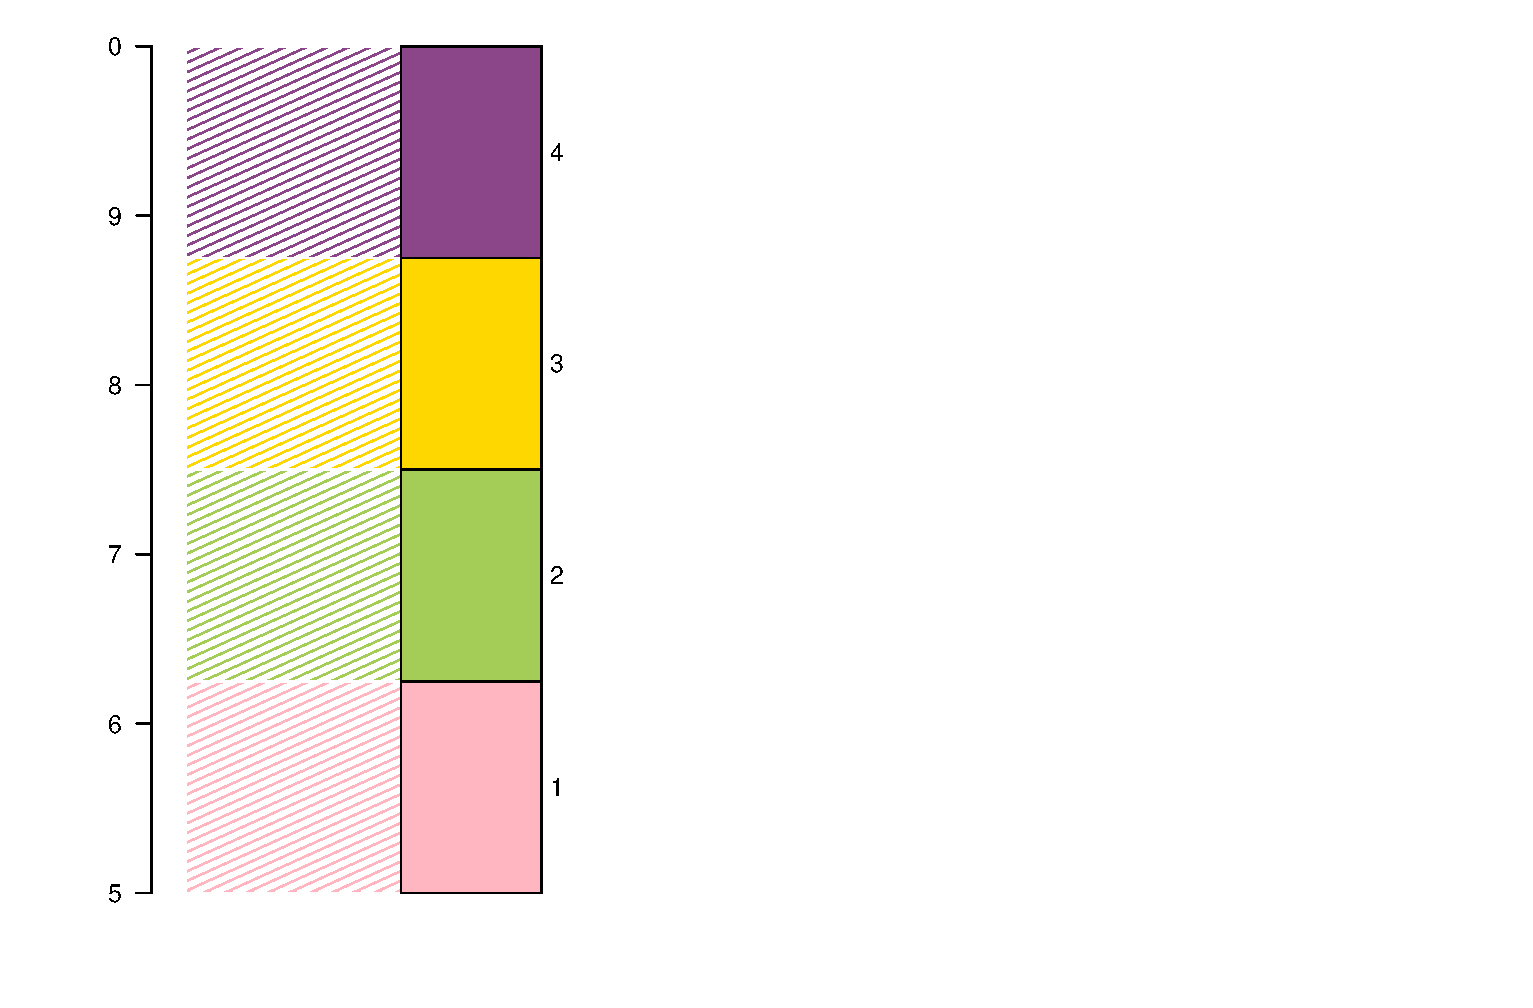
\includegraphics[width=6.5cm]{../figures/legend1}}
}

\psfrag{A}[l][c]{\miniscule{\begin{tabular}{@{}l@{}}
   \emph{One person household}---A single person \\
   living alone. This is defined the same in both \\
    typologies presented here. 
\end{tabular}}}
\psfrag{B}[l][c]{\miniscule{\begin{tabular}{@{}l@{}}
   \emph{One generation household}---at least one more\\
   person of the same age group as  the head\\
   Usually a spouse, but can also be sibling etc.
\end{tabular}}}

\psfrag{C}[l][c]{\miniscule{\begin{tabular}{@{}l@{}}
   \emph{Two generation household}---at least one more\\
   person one generation younger/older than the\\
   head. Usually child(ren),  can also be parent etc.
\end{tabular}}}

\psfrag{D}[l][c]{\miniscule{\begin{tabular}{@{}l@{}}
   \emph{Three or more generation household}---at least two\\
   more persons of different generations than the\\
   head (but without skipping generations). 
\end{tabular}}}


\psfrag{E}[l][c]{\miniscule{\begin{tabular}{@{}l@{}}
   \emph{Skipped generation household}---at least one \\
   generation missing. Usually head with \\
   grandchildren but without children. 
\end{tabular}}}



\rput[bl](0,2.33){
\rput[bl](0,0){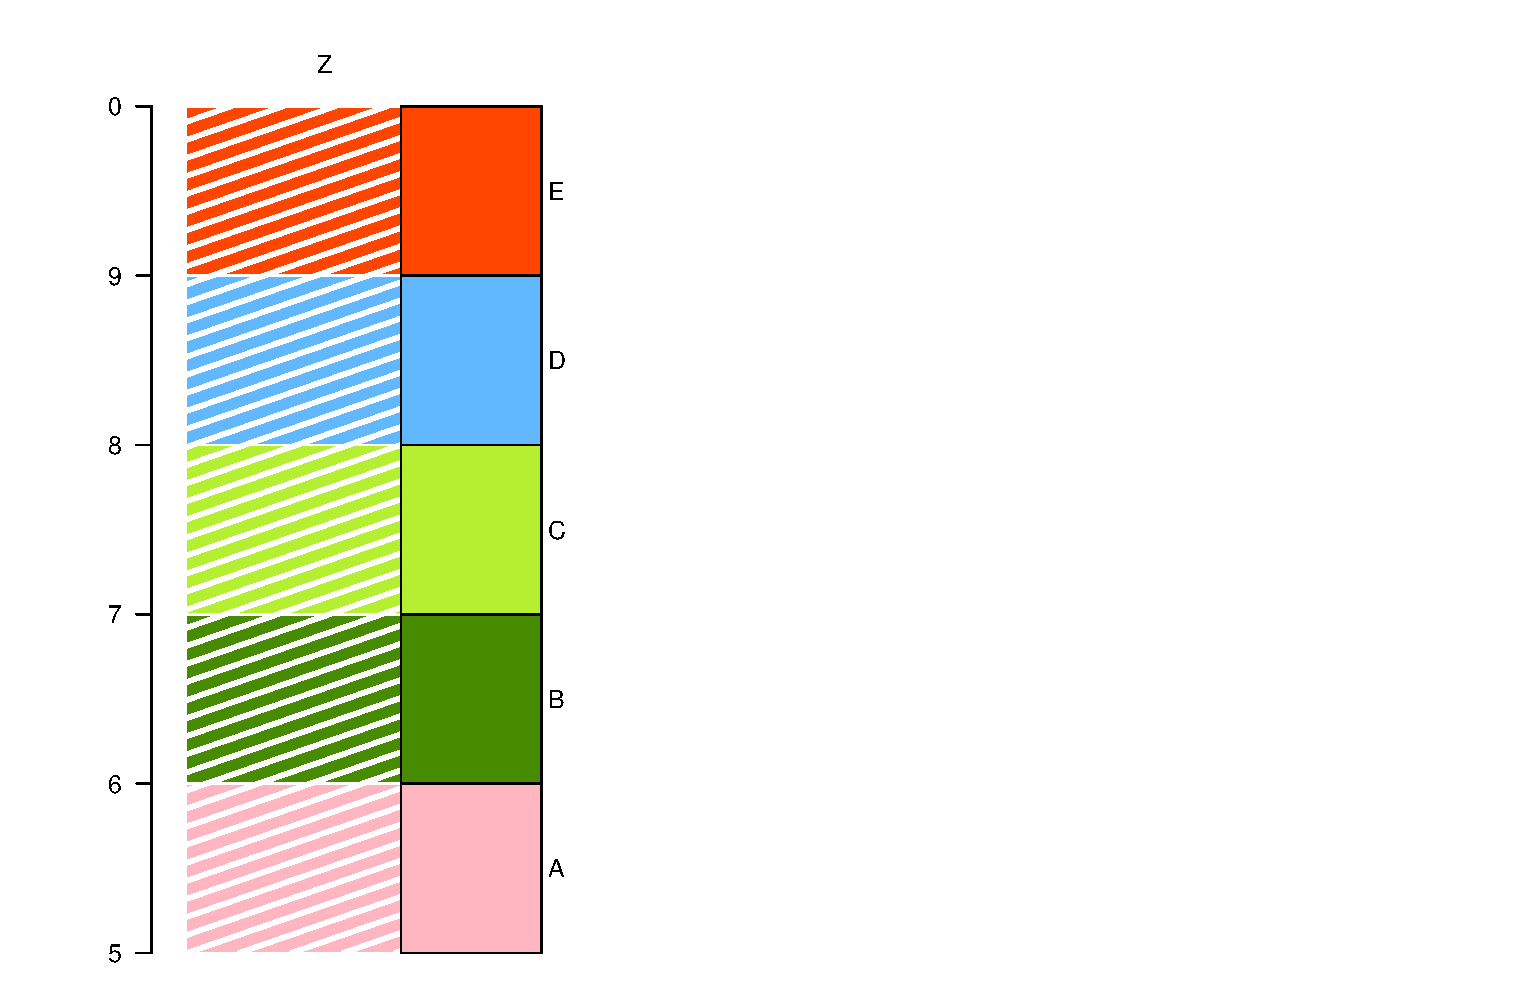
\includegraphics[width=6.5cm]{../figures/legend2}}

%\psframe(0,0)(1,2)
}

\rput[bl](1,3.33){
\rput[bl](0.0,0.01){
\mini{\parbox[c]
{7cm}{
\scriptsize \textsc{Legend}
\vspace{0.2em}

\minisculey 
In each chart the two typologies are presented side by side, for both men and women over 60. The lightly shaded background represents the distribution for the population as a whole. 
\vspace{0.5em}

The width of the two bars corresponds to the relative numbers of men and women over 60 years old, and their percentage is given underneath. All proportions are based on weighted counts with the total $N_{weighted}$ given above the chart.
\vspace{0.5em}

For definitions see legend descriptions to the left; the first set of household types uses UN recommended definitions for census data \citep{united1997}, while the second intergenerational structure is an \emph{ad hoc} typology.
 
}}}
}

\psfrag{5}[c][c]{\miniscule{0}}
\psfrag{6}[c][c]{\miniscule{0.2}}
\psfrag{7}[c][c]{\miniscule{0.4}}
\psfrag{8}[c][c]{\miniscule{0.6}}
\psfrag{9}[c][c]{\miniscule{0.8}}
\psfrag{0}[c][c]{\miniscule{1}}

\psfrag{A}[c][c]{\miniscule{Men}}
\psfrag{B}[c][c]{\miniscule{Women}}
\psfrag{1}[r][c]{\miniscule{\emph{One person}}}
\psfrag{2}[r][c]{\miniscule{\emph{Nuclear}}}
\psfrag{3}[r][c]{\miniscule{\emph{Extended}}}
\psfrag{4}[r][c]{\miniscule{\emph{Composite}}}




\psfrag{a}[l][c]{\miniscule{\emph{One person}}}
\psfrag{b}[l][c]{\miniscule{\emph{One gen.}}}
\psfrag{c}[l][c]{\miniscule{\emph{Two gen.}}}
\psfrag{d}[l][c]{\miniscule{\emph{Three+ gen.}}}
\psfrag{e}[l][c]{\miniscule{\emph{Skipped gen.}}}


\rput[bl](0,6.33){
\rput[bl](0.05,0.25){
\mini{\parbox[c]
{13.5cm}{

\maxi 
The prevalence of different household living arrangements varies across countries and across different population groups. This factsheet focuses on people over 60 years of age and compares men and women in each country. 
\textcolor{white}{\cite{gh2017}}
\vspace{1ex}

Using census microdata collected in the IPUMS-International database \citep{impus2017} we summarise the types of households in which older people live using  two typologies:
 \begin{itemize}
 \item the household composition based on family nuclei, and
 \item the intergenerational structure of the household. \end{itemize}  

The proportions displayed are of \emph{individuals} living in each type of household (not proportions of households of each type) and show important differences between genders, as well broader patterns that can be observed regionally and globally. The living arrangements of older people can also be contrasted to the average of the population as a whole, which is displayed as the background of each bar chart.

%In order to be able to distinguish multiple generations we selected countries where the \emph{relationship} variable  included grandchildren and grandparents, and limited the selection to census samples from this century. 
}}}
}




% 1,1
\rput[bl](0,0){
\psfrag{A}[c][b]{\miniscule{\begin{tabular}{@{}c@{}}
   \emph{Men}\\
   (4.86 \%)
\end{tabular}}}
\psfrag{B}[c][b]{\miniscule{\begin{tabular}{@{}c@{}}
   \emph{Women)}\\
   (5.64 \%)
\end{tabular}}}
\rput[bl](0,0){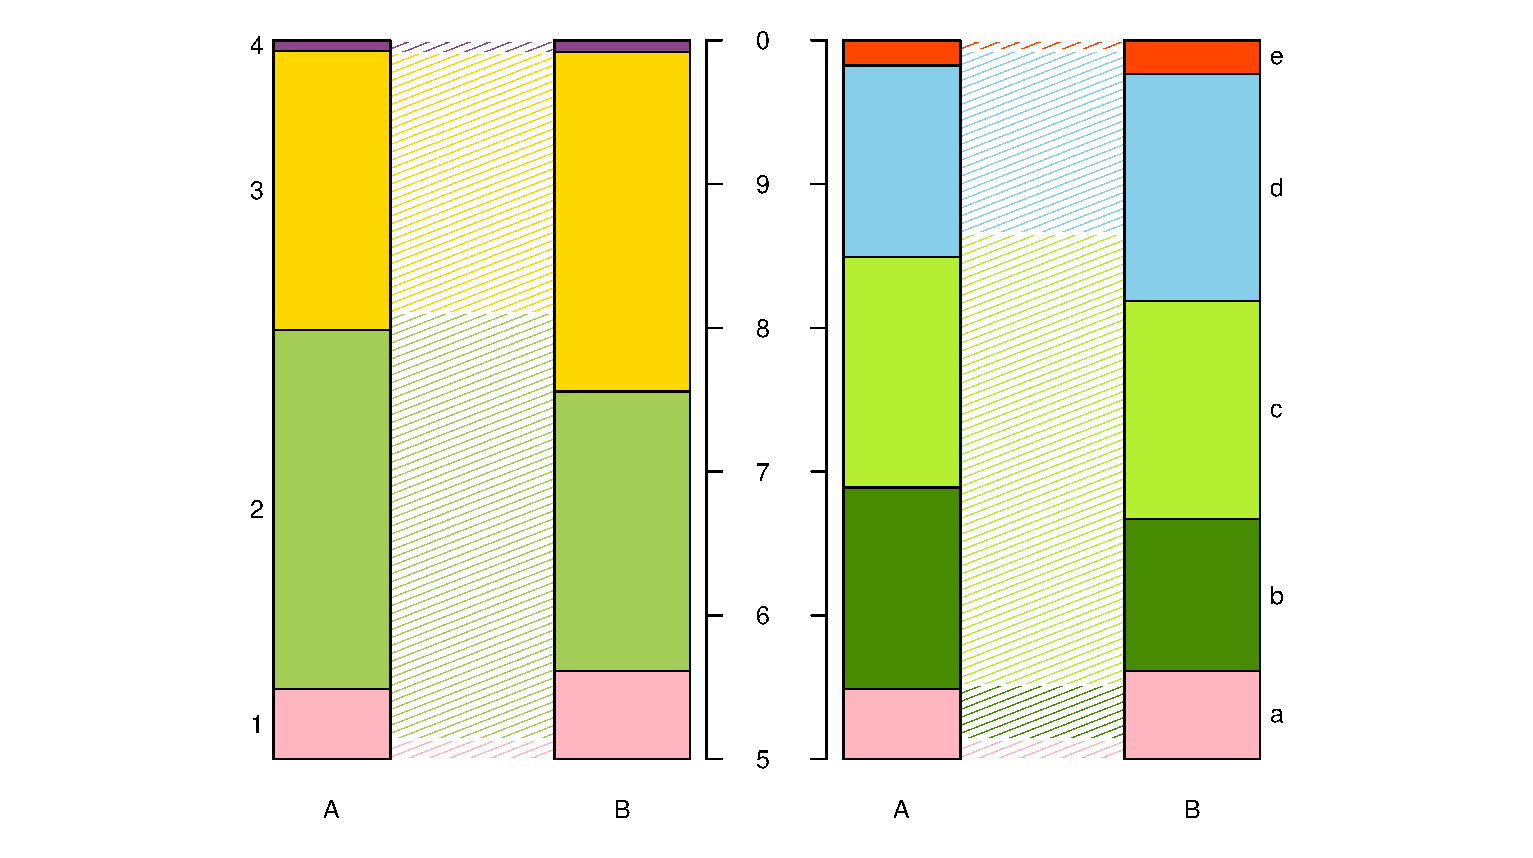
\includegraphics[width=7.425cm]{../figures/Mexico}}
\rput[bl](0.05,0.83) {\footnotesize  Mexico (2015) \miniscule $N_{weighted}=119,561,904 $}
%\psframe(0,0)(1,1)
}

\rput[bl](0.03,2.03){\large \textsc{Americas}
}
% 1,2
\rput[bl](0,1){
\psfrag{A}[c][b]{\miniscule{\begin{tabular}{@{}c@{}}
   \emph{Men}\\
   (6.93 \%)
\end{tabular}}}
\psfrag{B}[c][b]{\miniscule{\begin{tabular}{@{}c@{}}
   \emph{Women}\\
   (9.34 \%)
\end{tabular}}}
\rput[bl](0,0){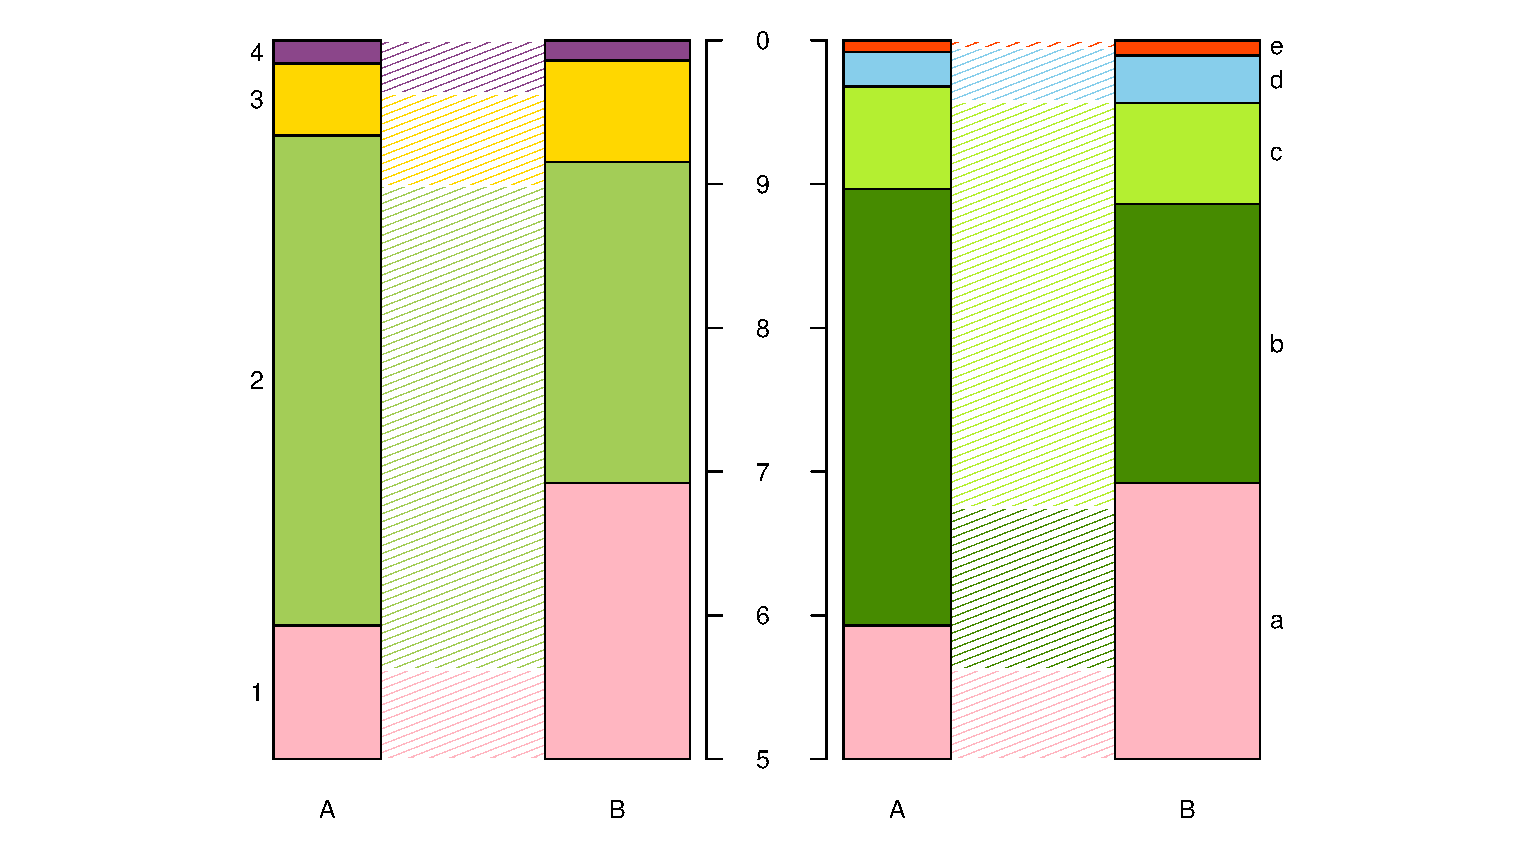
\includegraphics[width=7.425cm]{../figures/UnitedStates}}
\rput[bl](0.05,0.83) {\footnotesize United States (2000)\miniscule $N_{w}=281,421,906$}
%\psframe(0,0)(1,1)
}

% 2,1
\rput[bl](1,0){
\psfrag{A}[c][b]{\miniscule{\begin{tabular}{@{}c@{}}
   \emph{Men}\\
   (2.84 \%)
\end{tabular}}}
\psfrag{B}[c][b]{\miniscule{\begin{tabular}{@{}c@{}}
   \emph{Women}\\
   (3.22 \%)
\end{tabular}}}

\rput[bl](0,0){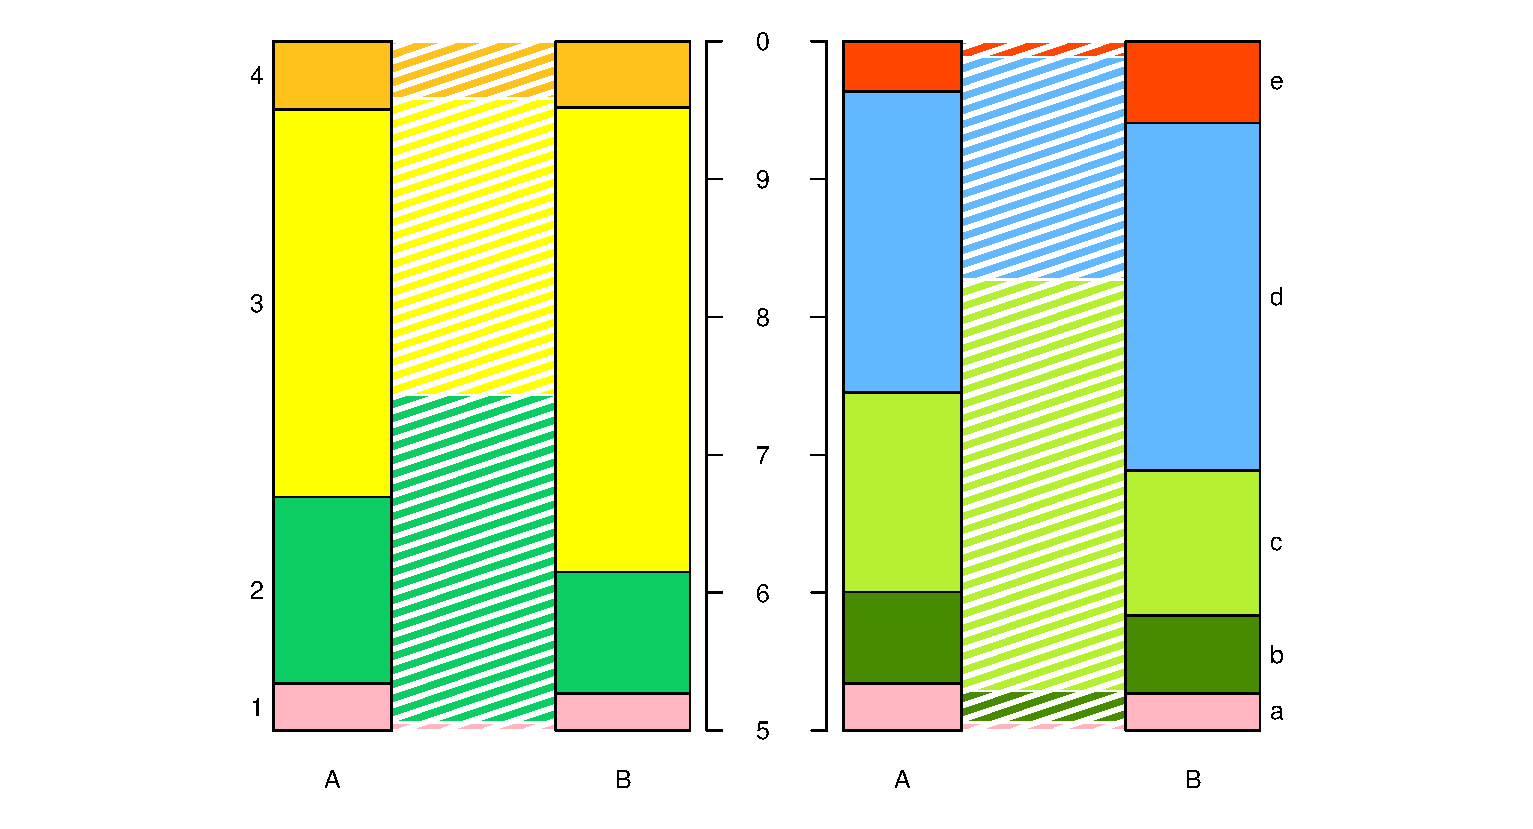
\includegraphics[width=7.425cm]{../figures/Nicaragua}}
\rput[bl](0.05,0.83) {\footnotesize Nicaragua (2005)\miniscule $N_{weighted}=5,154,850 $}
%\psframe(0,0)(1,1)
}

%2,2
% 1,2
\rput[bl](1,1){

\psfrag{A}[c][b]{\miniscule{\begin{tabular}{@{}c@{}}
   \emph{Men}\\
   (5.14 \%)
\end{tabular}}}
\psfrag{B}[c][b]{\miniscule{\begin{tabular}{@{}c@{}}
   \emph{Women}\\
   (5.48 \%)
\end{tabular}}}

\rput[bl](0,0){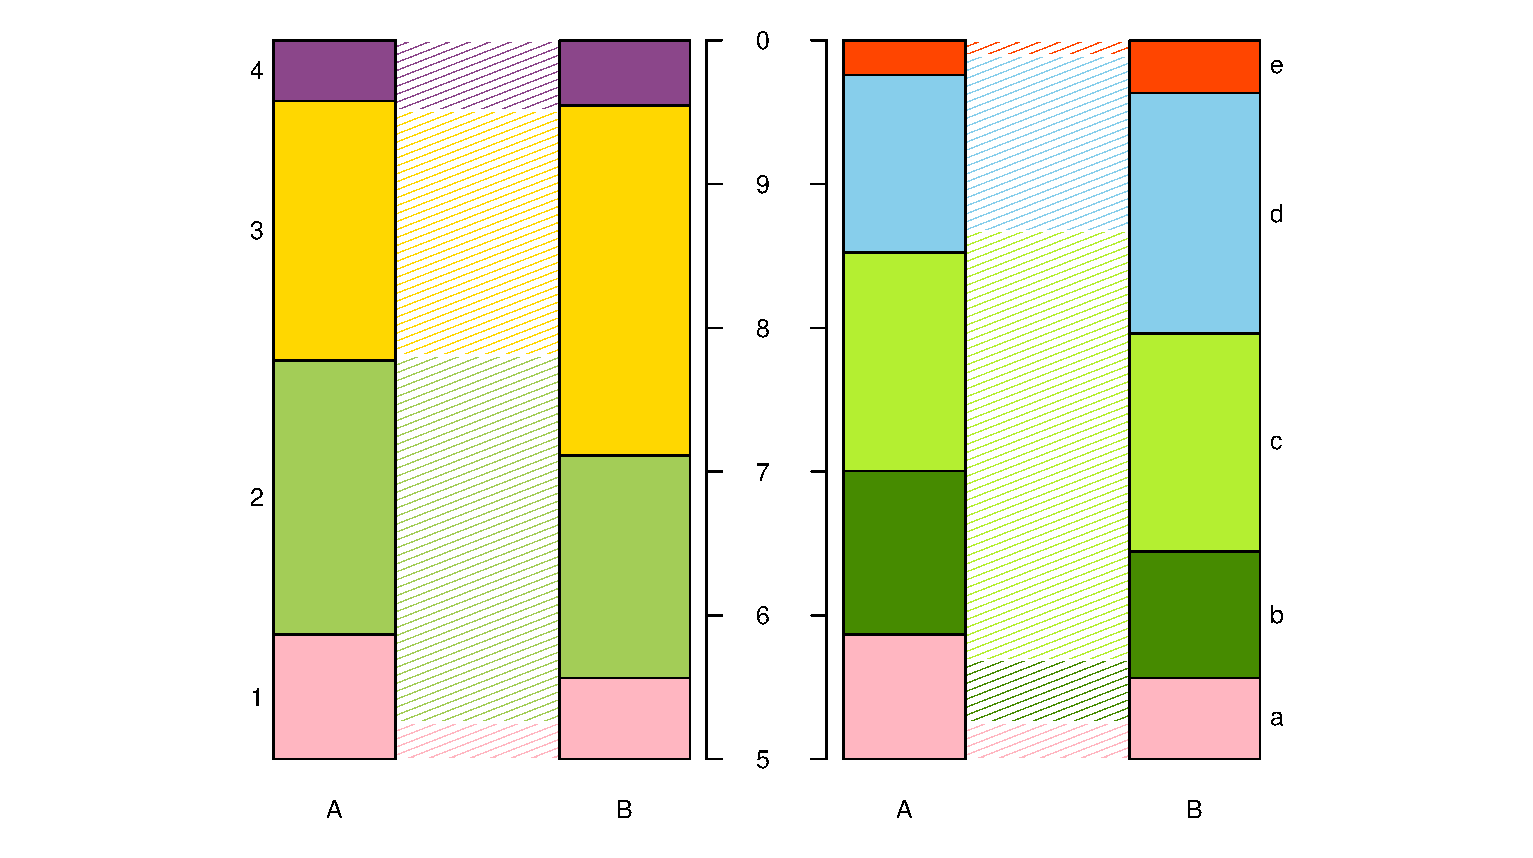
\includegraphics[width=7.425cm]{../figures/Panama}}
\rput[bl](0.05,0.83) {\footnotesize Panama (2010)\miniscule $N_{weighted}= 3,411,180 $}
%\psframe(0,0)(1,1)
}



\rput[bl](2,1){
\psfrag{A}[c][b]{\miniscule{\begin{tabular}{@{}c@{}}
   \emph{Men}\\
   (4.39 \%)
\end{tabular}}}
\psfrag{B}[c][b]{\miniscule{\begin{tabular}{@{}c@{}}
   \emph{Women}\\
   (4.68 \%)
\end{tabular}}}

\rput[bl](0,0){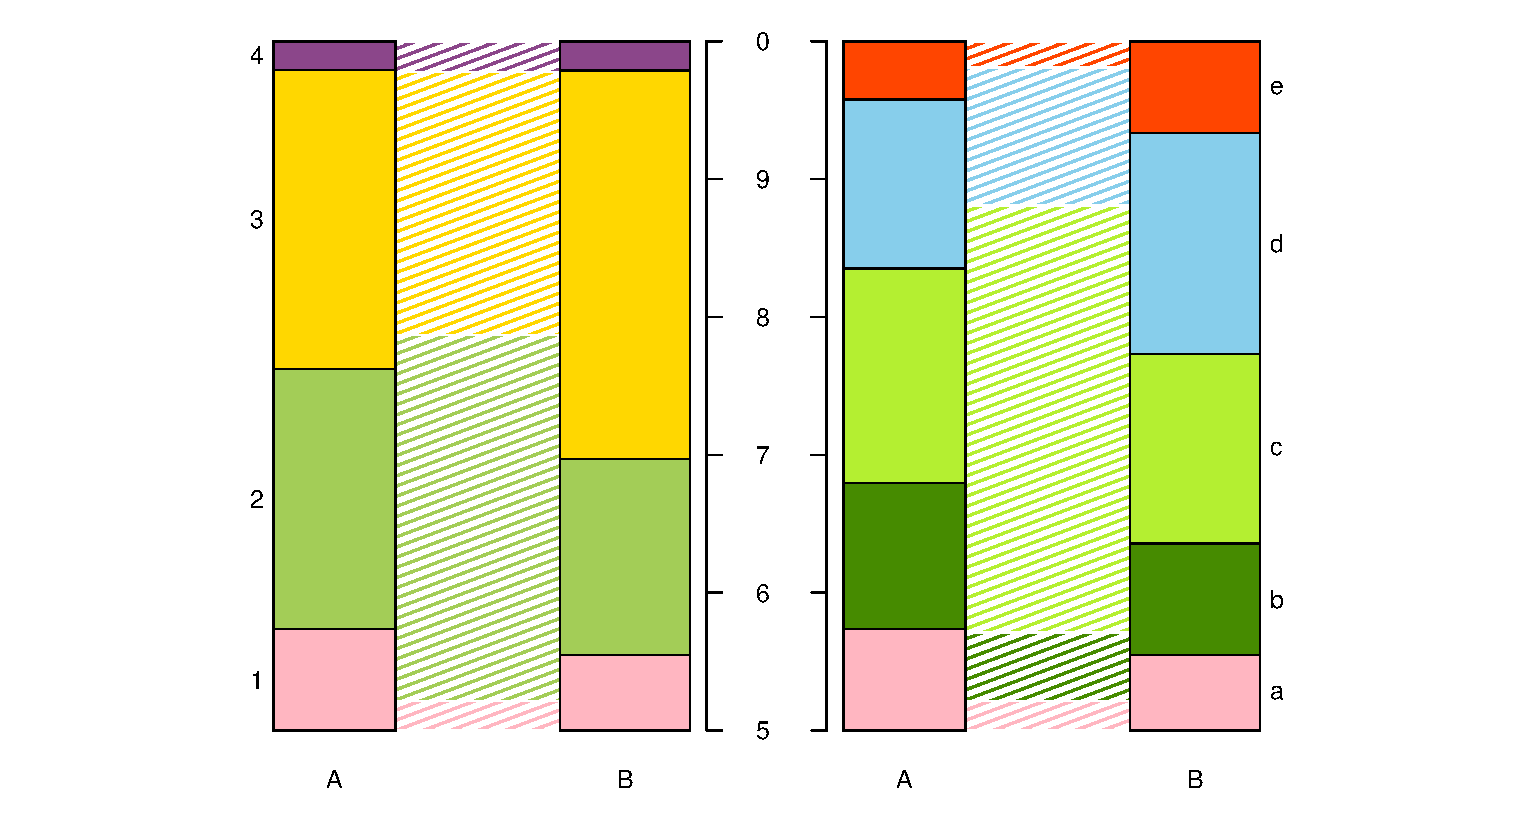
\includegraphics[width=7.425cm]{../figures/DominicanRepublic}}
\rput[bl](0.05,0.83) {\footnotesize Dominican Rep.(2010)\miniscule $N_{w}=9,437,840$}
%\psframe(0,0)(1,1)
}

\rput[bl](2,0){
\psfrag{A}[c][b]{\miniscule{\begin{tabular}{@{}c@{}}
   \emph{Men}\\
   (6.76 \%)
\end{tabular}}}
\psfrag{B}[c][b]{\miniscule{\begin{tabular}{@{}c@{}}
   \emph{Women}\\
   (8.59 \%)
\end{tabular}}}
\rput[bl](0,0){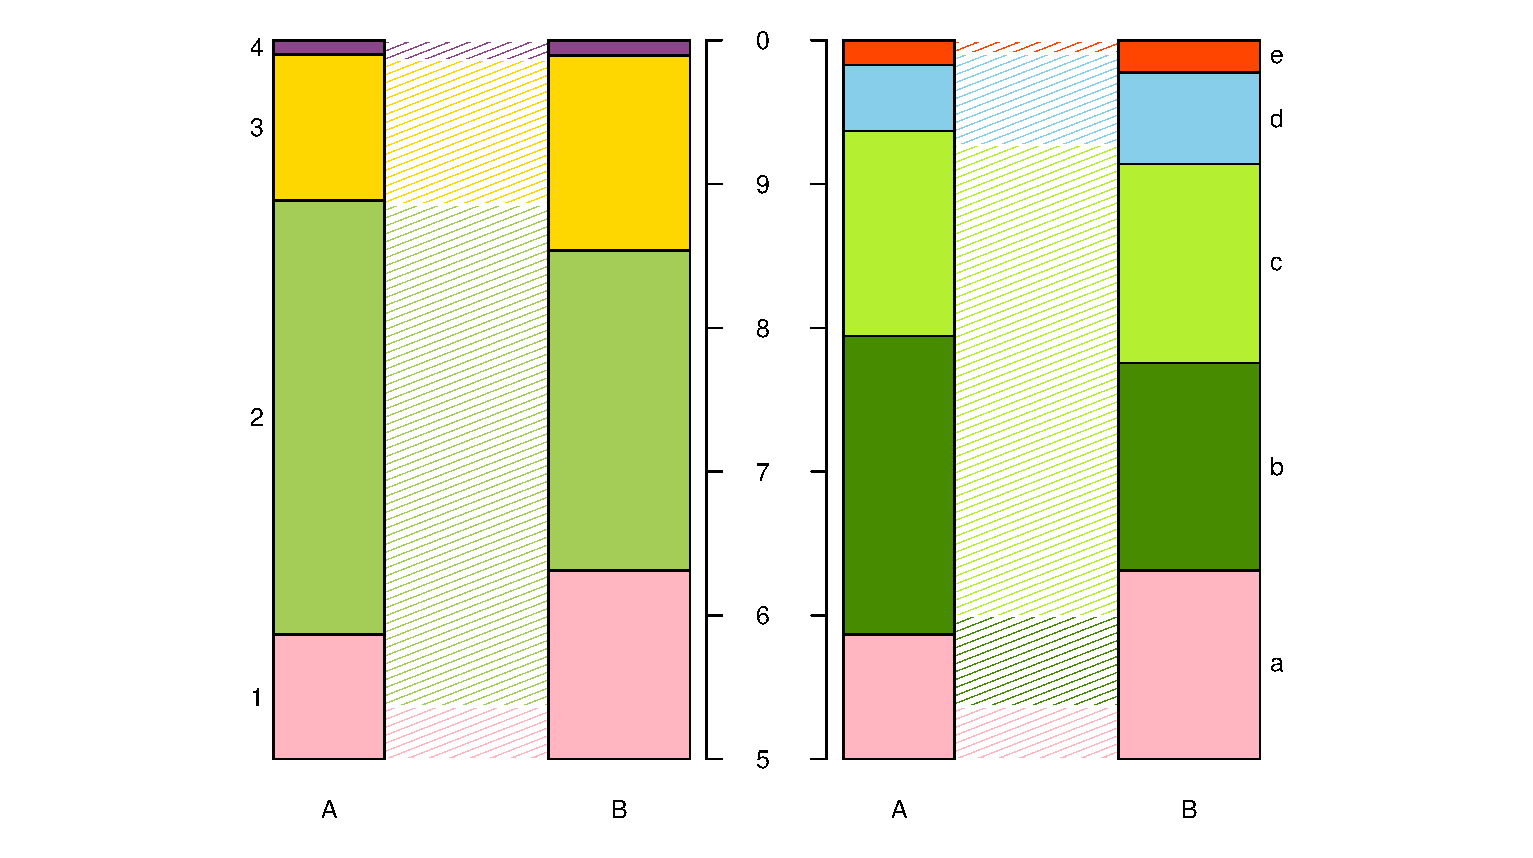
\includegraphics[width=7.425cm]{../figures/PuertoRico}}
\rput[bl](0.05,0.83) {\footnotesize Puerto Rico (2000)\miniscule $N_{w} = 3,808,610$}
%\psframe(0,0)(1,1)
}

\rput[bl](3,1){
\psfrag{A}[c][b]{\miniscule{\begin{tabular}{@{}c@{}}
   \emph{Men}\\
   (4.80 \%)
\end{tabular}}}
\psfrag{B}[c][b]{\miniscule{\begin{tabular}{@{}c@{}}
   \emph{Women}\\
   (6.00 \%)
\end{tabular}}}
\rput[bl](0,0){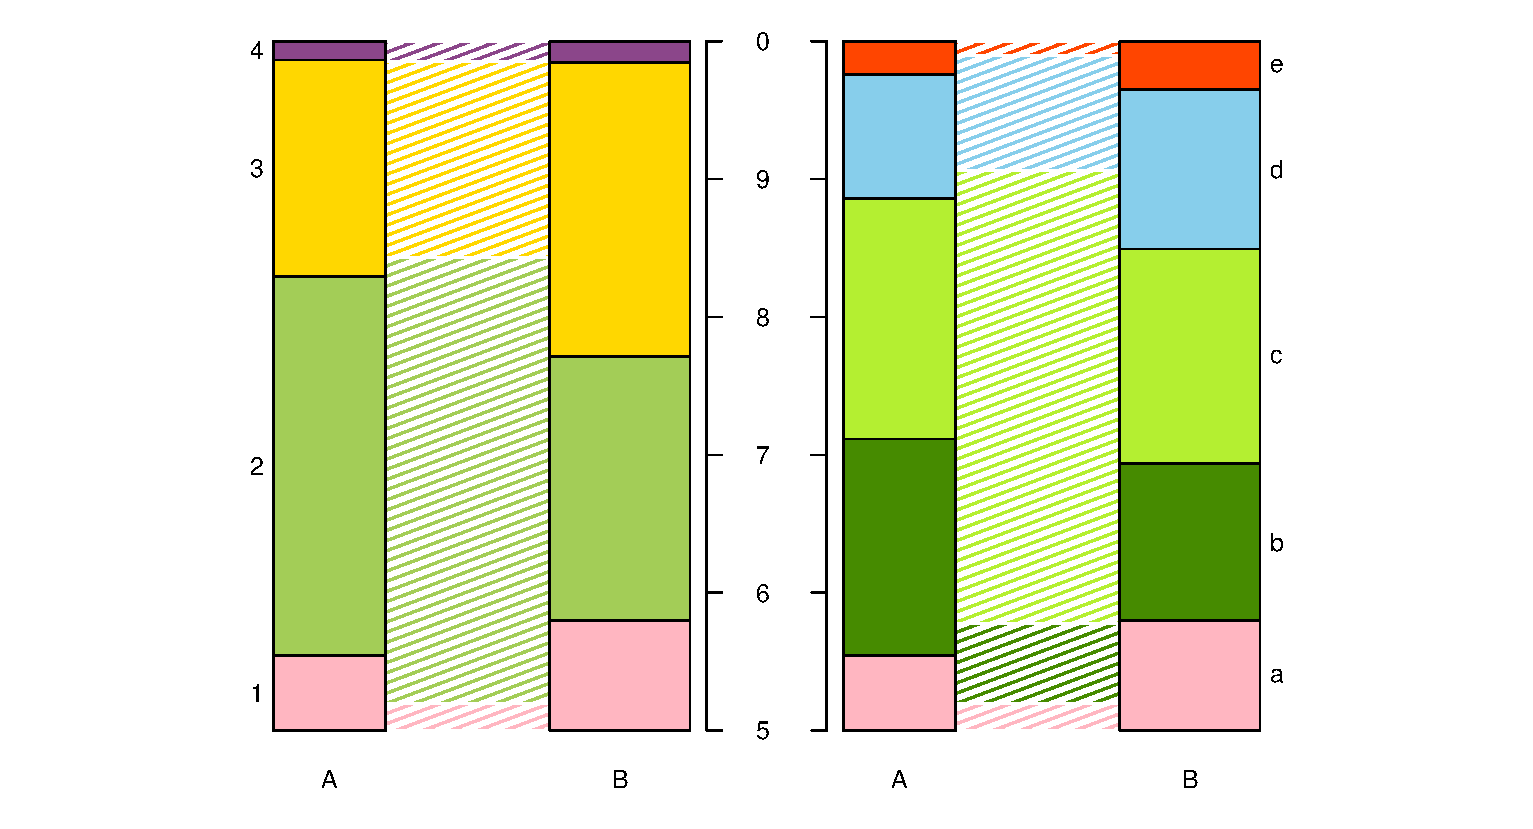
\includegraphics[width=7.425cm]{../figures/Brazil}}
\rput[bl](0.05,0.83) {\footnotesize Brazil (2010) \miniscule $N_{weighted} =190,822,749$}
%\psframe(0,0)(1,1)
}


\rput[bl](1,2.33){
\psfrag{A}[c][b]{\miniscule{\begin{tabular}{@{}c@{}}
   \emph{Men}\\
   (6.05 \%)
\end{tabular}}}
\psfrag{B}[c][b]{\miniscule{\begin{tabular}{@{}c@{}}
   \emph{Women}\\
   (8.65 \%)
\end{tabular}}}
\rput[bl](0,0){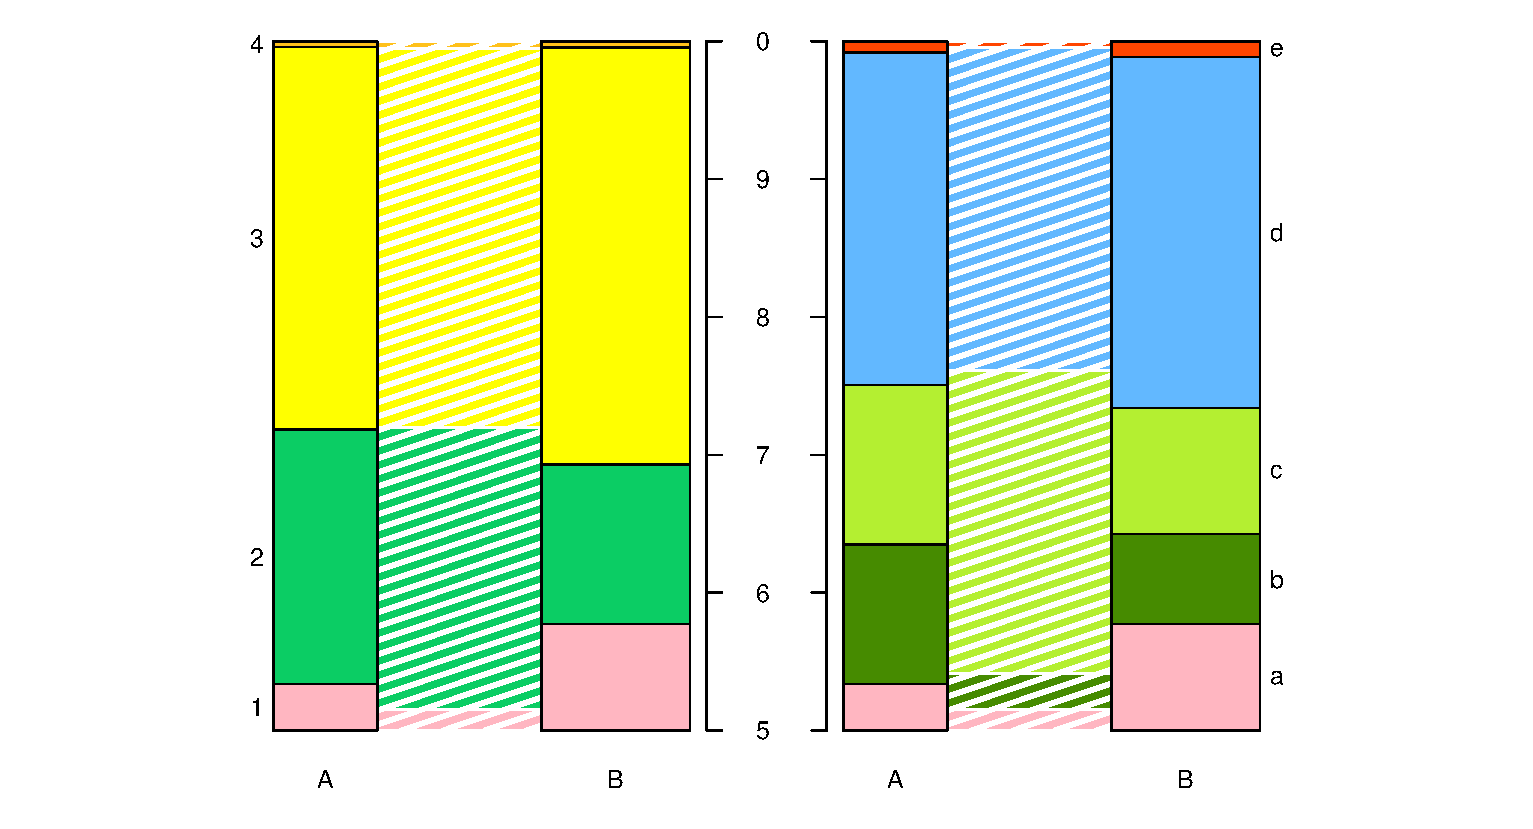
\includegraphics[width=7.425cm]{../figures/Armenia}}
\rput[bl](0.05,0.83) {\footnotesize Armenia (2011) \miniscule $N_{weighted} = 3,018,310$ }
%\psframe(0,0)(1,1)
}
 
\rput[bl](3,2.33){
\psfrag{A}[c][b]{\miniscule{\begin{tabular}{@{}c@{}}
   \emph{Men}\\
   (2.64 \%)
\end{tabular}}}
\psfrag{B}[c][b]{\miniscule{\begin{tabular}{@{}c@{}}
   \emph{Women}\\
   (3.78 \%)
\end{tabular}}}
\rput[bl](0,0){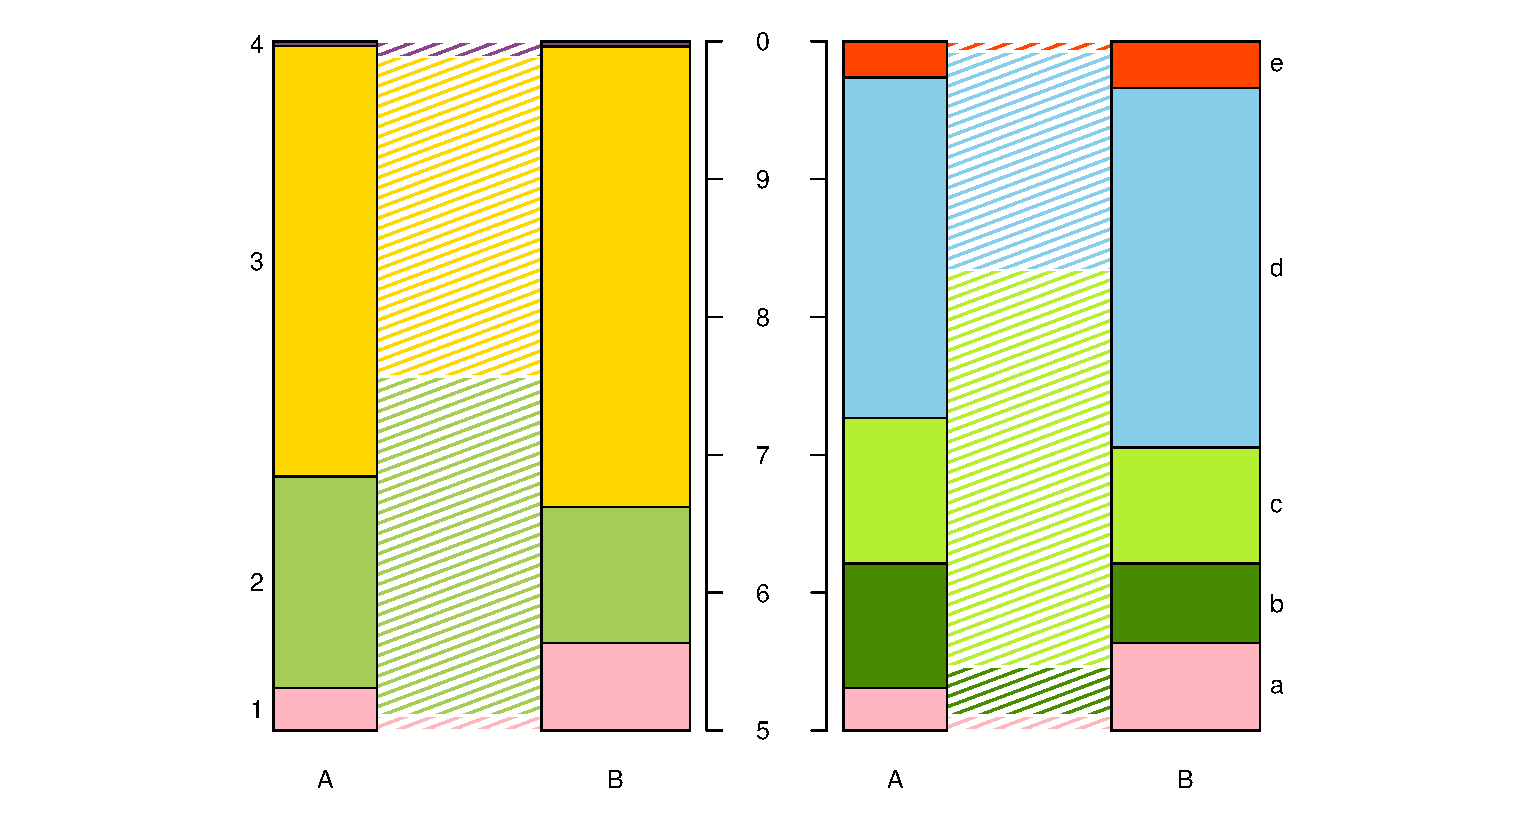
\includegraphics[width=7.425cm]{../figures/KyrgyzRepublic}}
\rput[bl](0.05,0.83) {\footnotesize Kyrgyz Rep.(2009)\miniscule $N_{w} = 5,649,860 $}
%\psframe(0,0)(1,1)
} 
\rput[bl](2,2.33){
\psfrag{A}[c][b]{\miniscule{\begin{tabular}{@{}c@{}}
   \emph{Men}\\
   (3.39 \%)
\end{tabular}}}
\psfrag{B}[c][b]{\miniscule{\begin{tabular}{@{}c@{}}
   \emph{Women}\\
   (3.87 \%)
\end{tabular}}}

\rput[bl](0,0){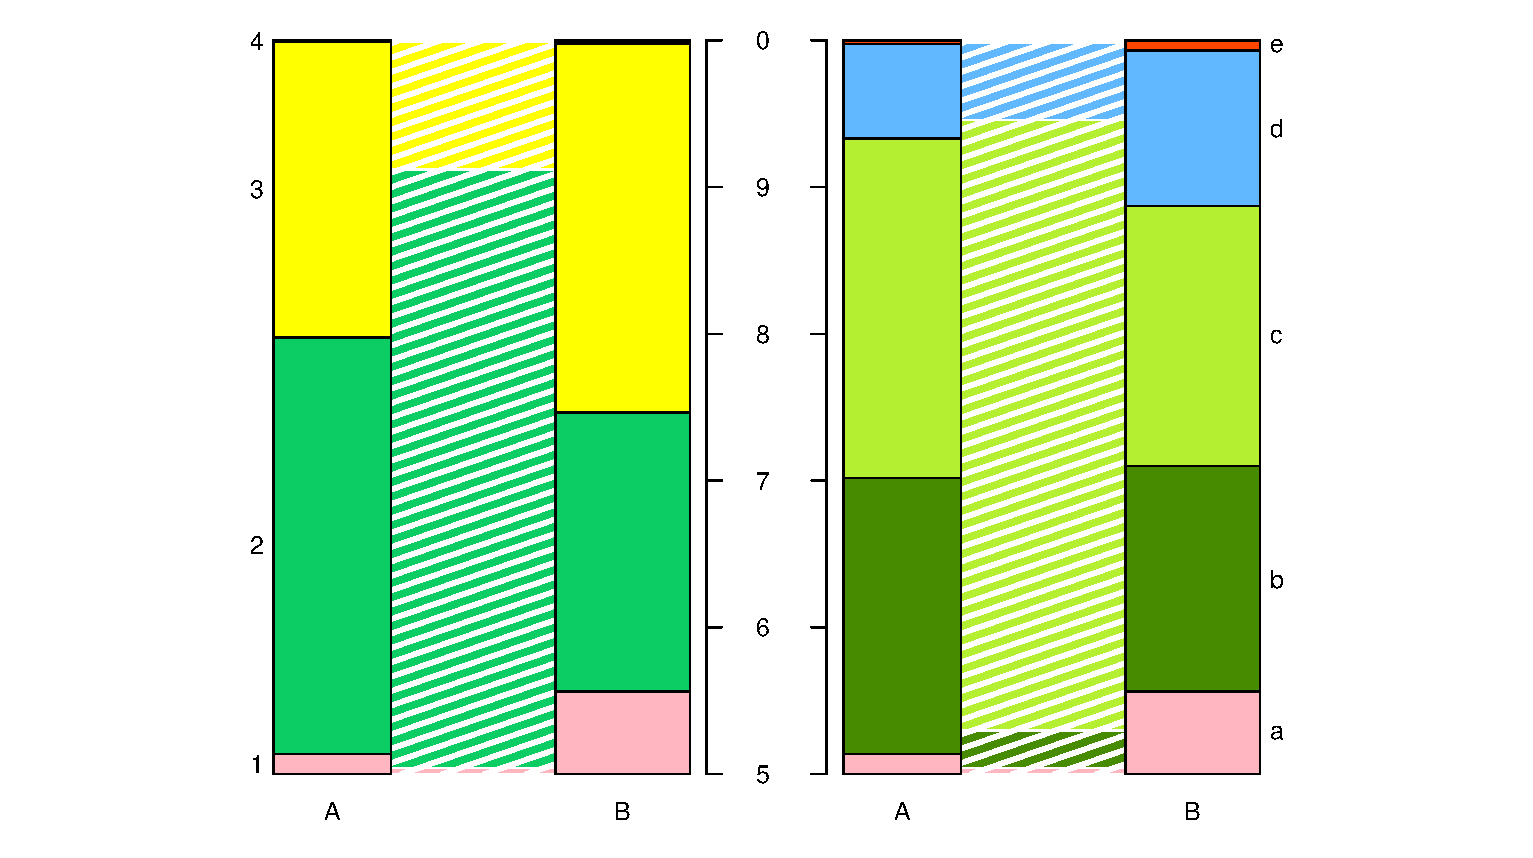
\includegraphics[width=7.425cm]{../figures/Palestine}}
\rput[bl](0.05,0.83) {\footnotesize Palestine (2007)\miniscule $N_{weighted}=2,188,173$}
%\psframe(0,0)(1,1)
} 

\rput[bl](2,3.33){
\psfrag{A}[c][b]{\miniscule{\begin{tabular}{@{}c@{}}
   \emph{Men}\\
   (5.28 \%)
\end{tabular}}}
\psfrag{B}[c][b]{\miniscule{\begin{tabular}{@{}c@{}}
   \emph{Women}\\
   (5.56\%)
\end{tabular}}}
\rput[bl](0,0){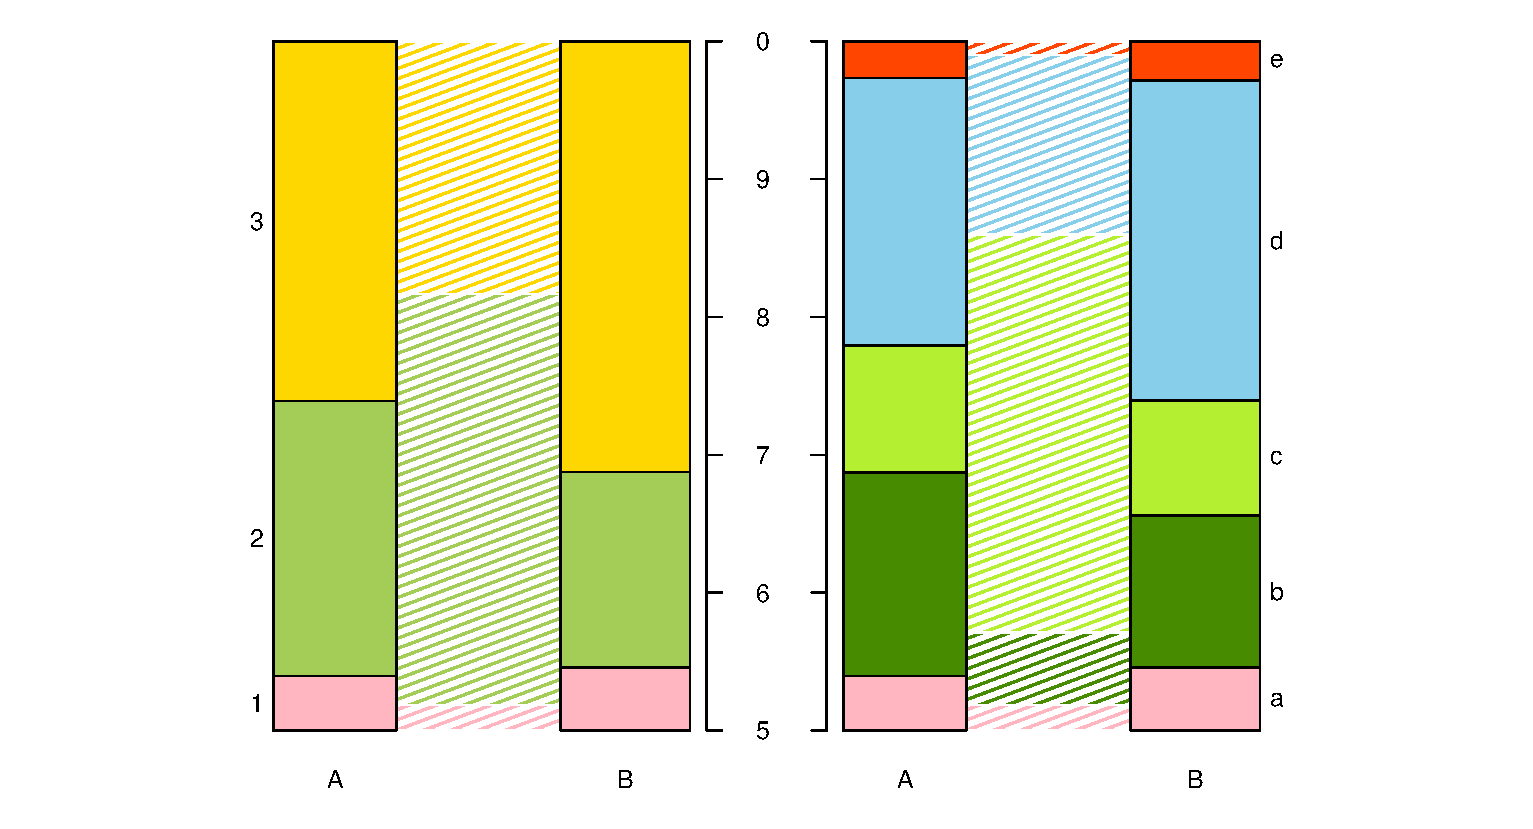
\includegraphics[width=7.425cm]{../figures/China}}
\rput[bl](0.05,0.83) {\footnotesize China (2000)\miniscule $N_{weighted} =1,180,434,400 $}
%\psframe(0,0)(1,1)
} 

\rput[bl](3,3.33){
\psfrag{A}[c][b]{\miniscule{\begin{tabular}{@{}c@{}}
   \emph{Men}\\
   (2.31 \%)
\end{tabular}}}
\psfrag{B}[c][b]{\miniscule{\begin{tabular}{@{}c@{}}
   \emph{Women}\\
   (2.98 \%)
\end{tabular}}}
\rput[bl](0,0){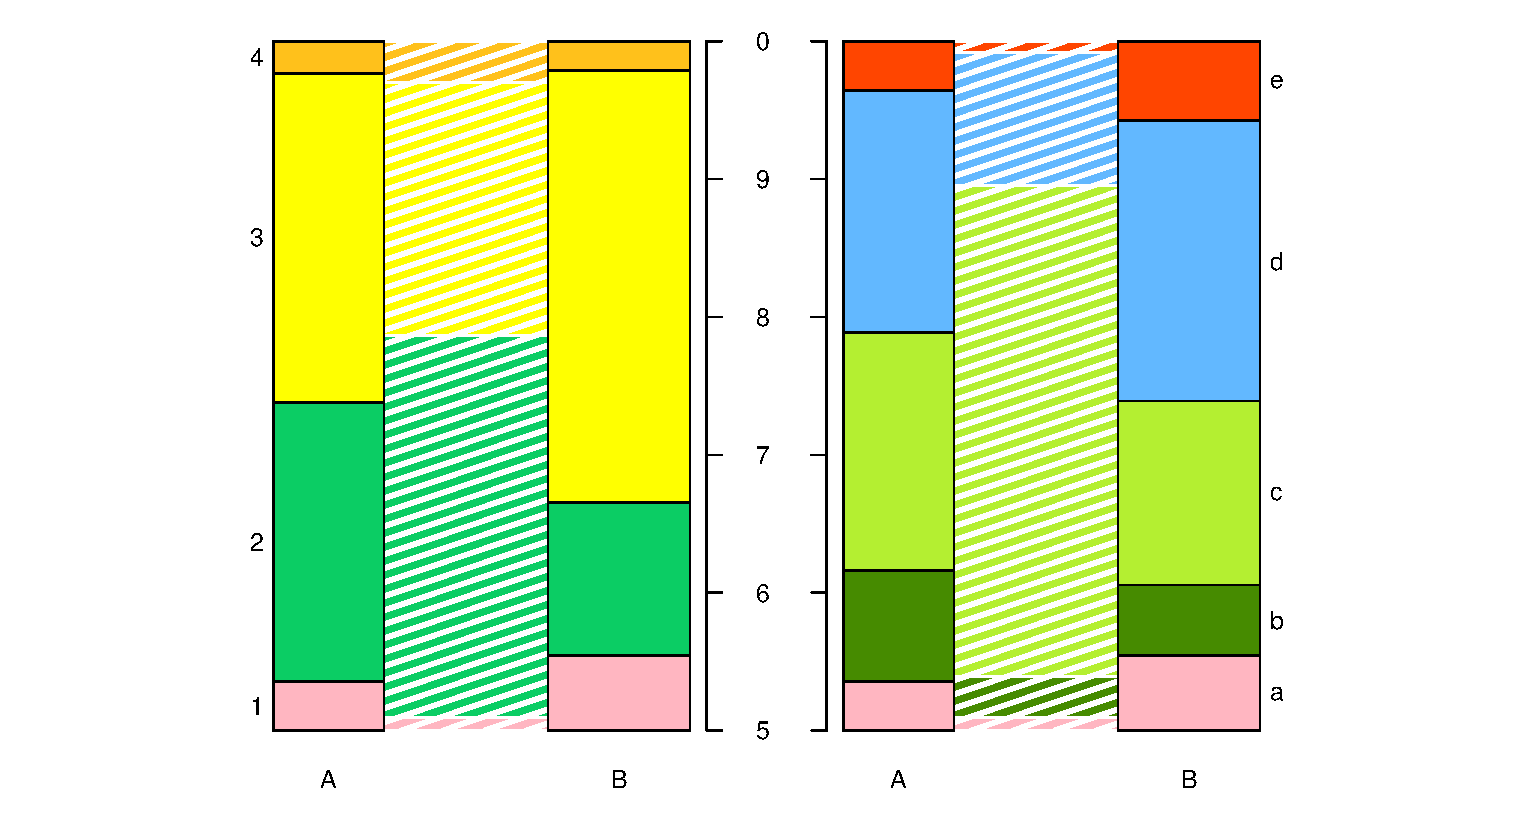
\includegraphics[width=7.425cm]{../figures/Mongolia}}
\rput[bl](0.05,0.83) {\footnotesize Mongolia(2000) \miniscule $N_{weighted}=2,437,250 $}
%\psframe(0,0)(1,1)
} 
\rput[bl](2.03,4.36){\large \textsc{Asia}
}

\rput[bl](3,4.66){
\psfrag{A}[c][b]{\miniscule{\begin{tabular}{@{}c@{}}
   \emph{Men}\\
   (8.33 \%)
\end{tabular}}}
\psfrag{B}[c][b]{\miniscule{\begin{tabular}{@{}c@{}}
   \emph{Women}\\
   (11.21 \%)
\end{tabular}}}
\rput[bl](0,0){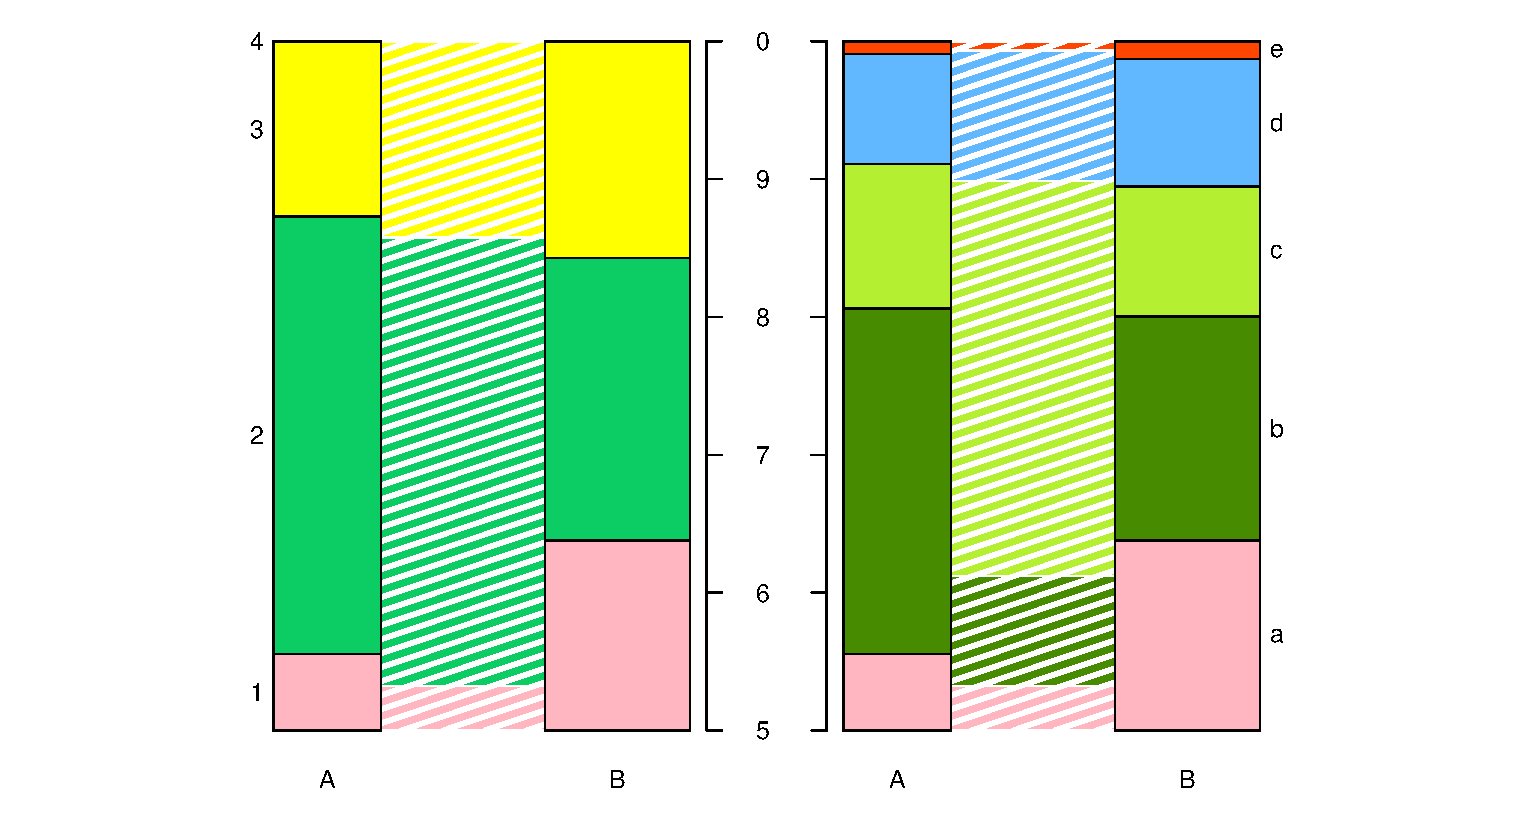
\includegraphics[width=7.425cm]{../figures/Romania}}
\rput[bl](0.05,0.83) {\footnotesize Romania (2002)\miniscule $N_{weighted}= 21,379,670$}
%\psframe(0,0)(1,1)
} 

\rput[bl](2,4.66){
\psfrag{A}[c][b]{\miniscule{\begin{tabular}{@{}c@{}}
   \emph{Men}\\
   (10.79\%)
\end{tabular}}}
\psfrag{B}[c][b]{\miniscule{\begin{tabular}{@{}c@{}}
   \emph{Women}\\
   (14.22 \%)
\end{tabular}}}
\rput[bl](0,0){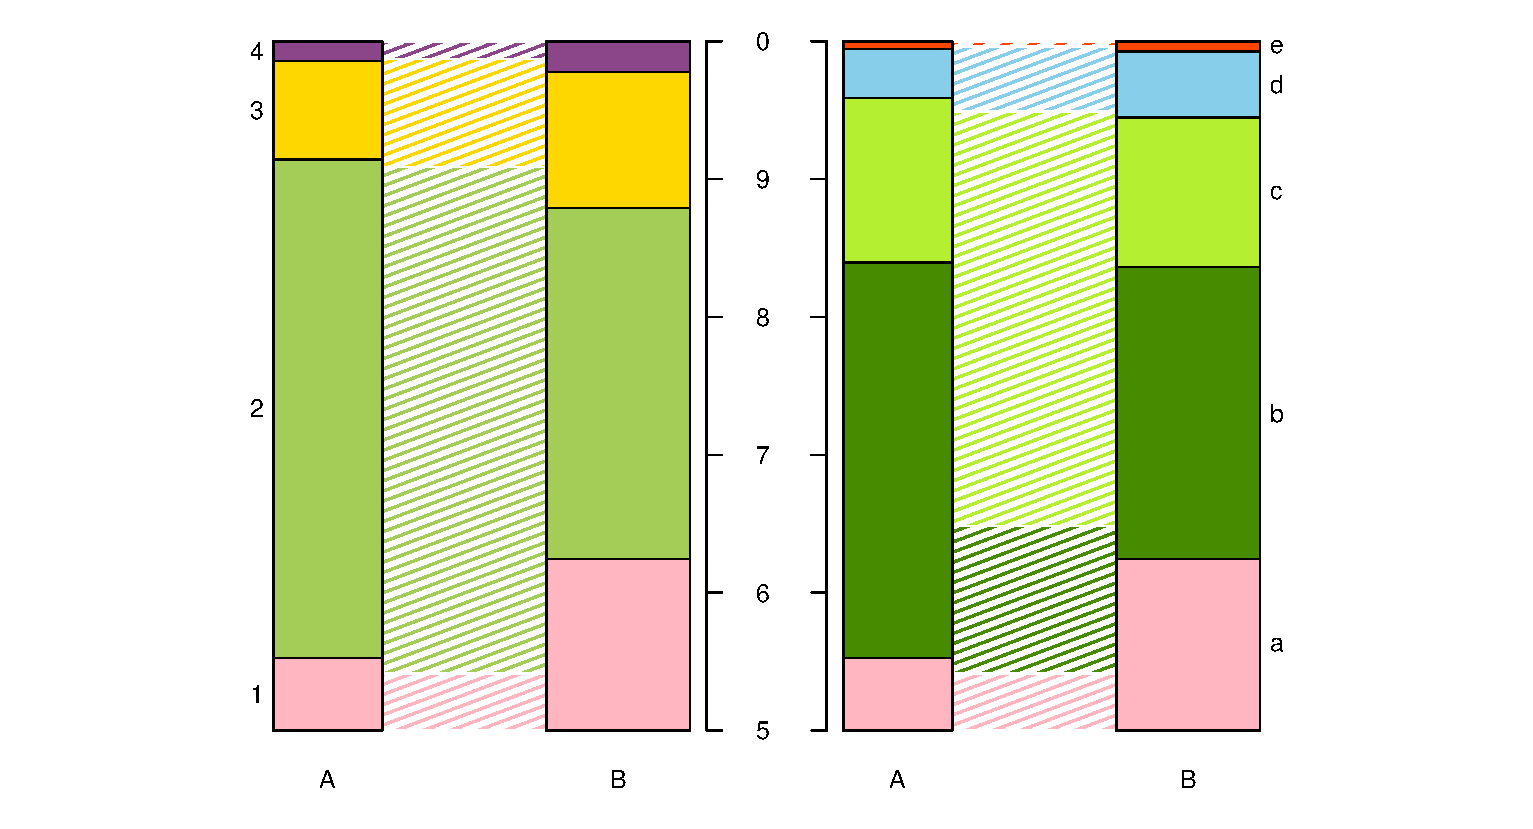
\includegraphics[width=7.425cm]{../figures/Portugal}}
\rput[bl](0.05,0.83) {\footnotesize Portugal (2011)\miniscule $N_{weighted} = 10,577,400$}
%\psframe(0,0)(1,1)
} 
\rput[bl](3,5.66){
\psfrag{A}[c][b]{\miniscule{\begin{tabular}{@{}c@{}}
   \emph{Men}\\
   (6.74 \%)
\end{tabular}}}
\psfrag{B}[c][b]{\miniscule{\begin{tabular}{@{}c@{}}
   \emph{Women}\\
   (10.22 \%)
\end{tabular}}}
\rput[bl](0,0){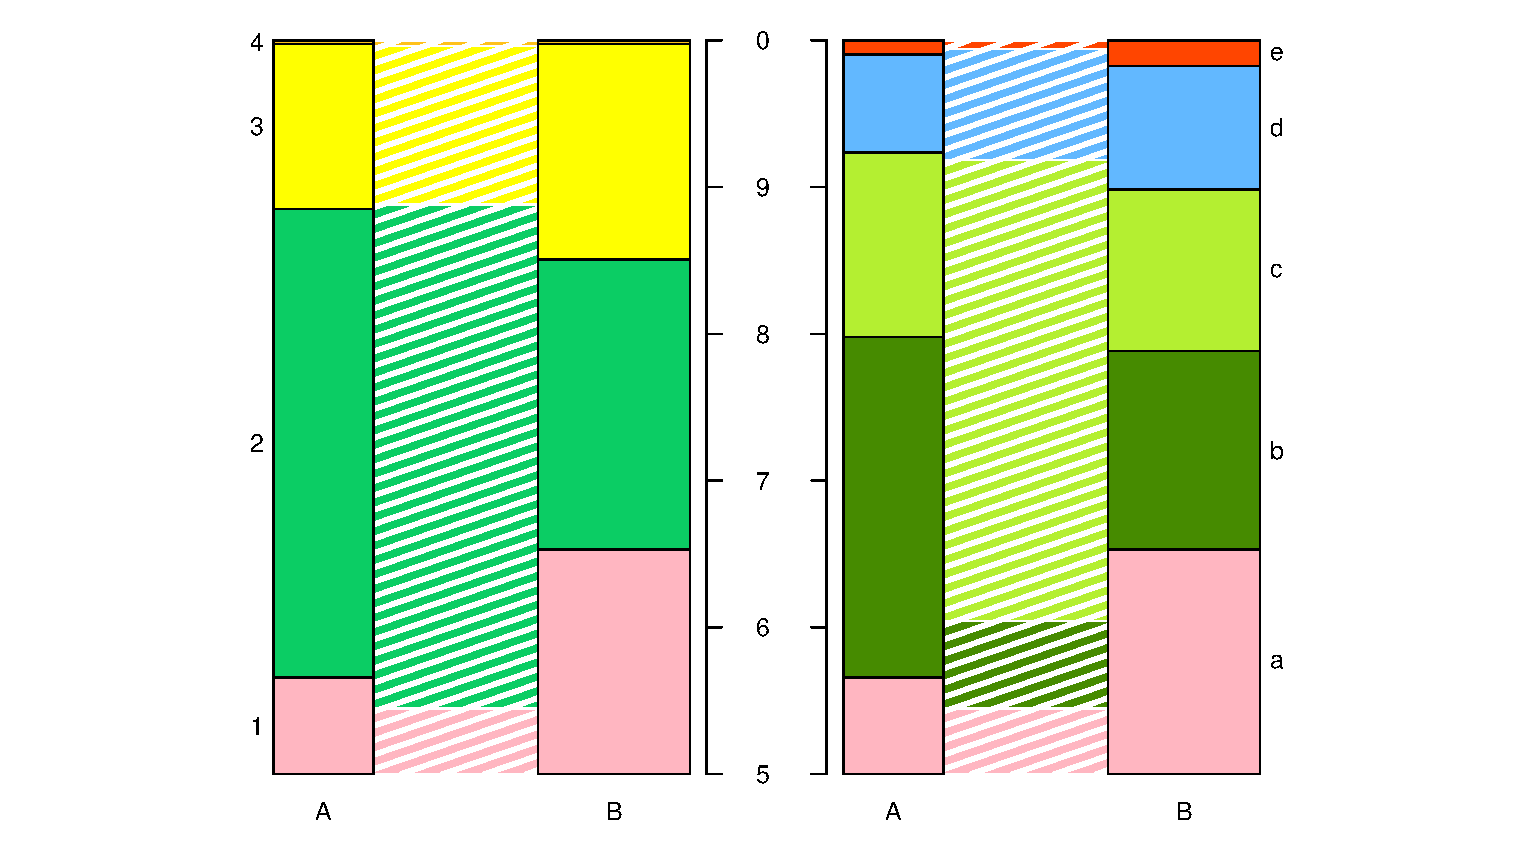
\includegraphics[width=7.425cm]{../figures/Poland}}
\rput[bl](0.05,0.83) {\footnotesize Poland (2002)\miniscule $N_{weighted} = 38,240,560 $}
%\psframe(0,0)(1,1)
} 
\rput[bl](3,6.66){
\psfrag{A}[c][b]{\miniscule{\begin{tabular}{@{}c@{}}
   \emph{Men}\\
   (6.60 \%)
\end{tabular}}}
\psfrag{B}[c][b]{\miniscule{\begin{tabular}{@{}c@{}}
   \emph{Women}\\
   (12.40 \%)
\end{tabular}}}
\rput[bl](0,0){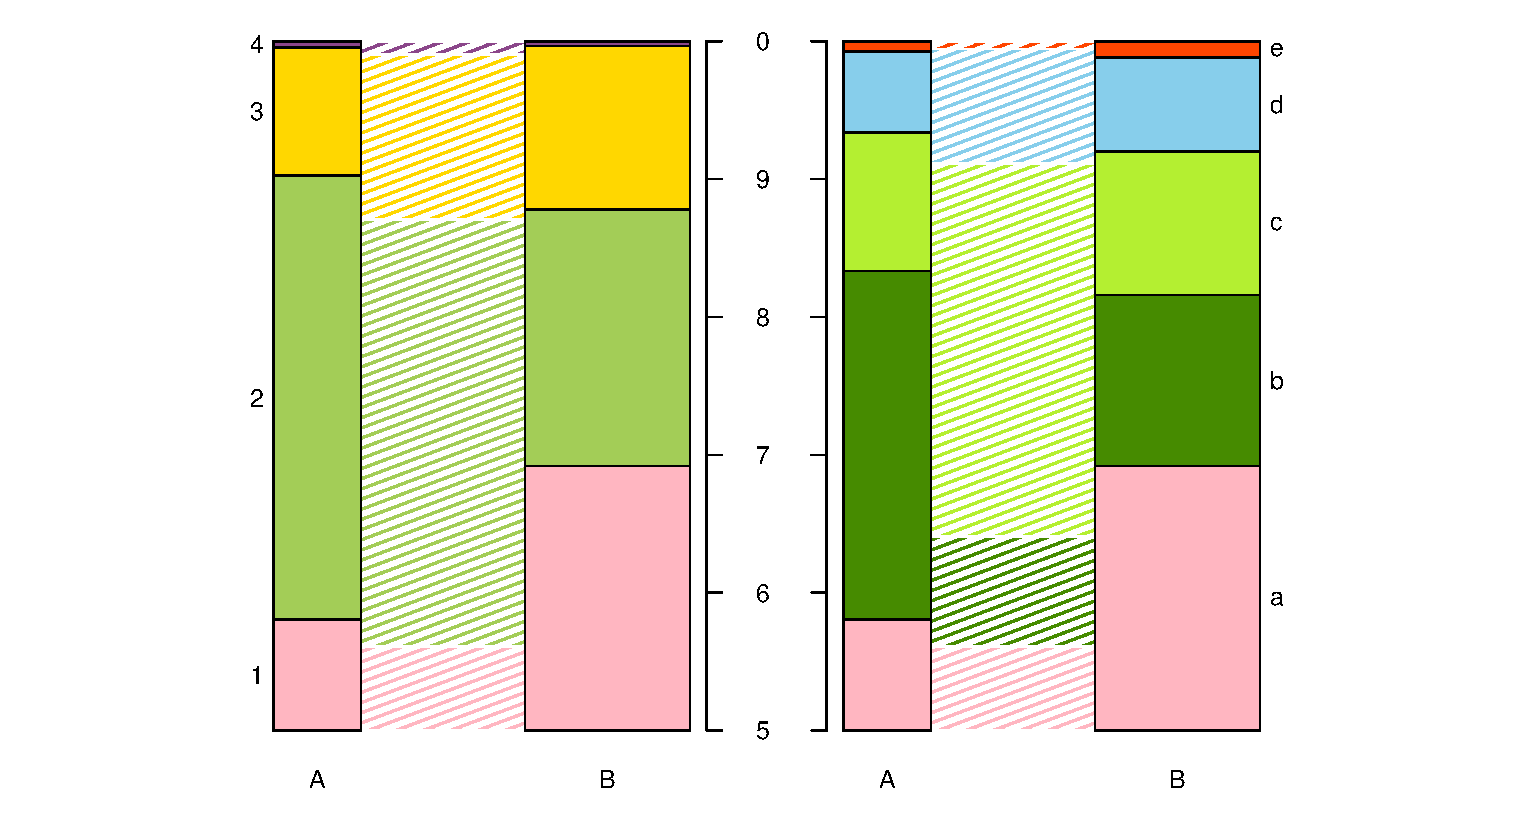
\includegraphics[width=7.425cm]{../figures/Belarus}}
\rput[bl](0.05,0.83) {\footnotesize Belarus (2009) \miniscule $N_{weighted}=9,405,940$}
%\psframe(0,0)(1,1)
} 

\rput[bl](2,6.66){
\psfrag{A}[c][b]{\miniscule{\begin{tabular}{@{}c@{}}
   \emph{Men}\\
   (7.50 \%)
\end{tabular}}}
\psfrag{B}[c][b]{\miniscule{\begin{tabular}{@{}c@{}}
   \emph{Women}\\
   (8.60 \%)
\end{tabular}}}
\rput[bl](0,0){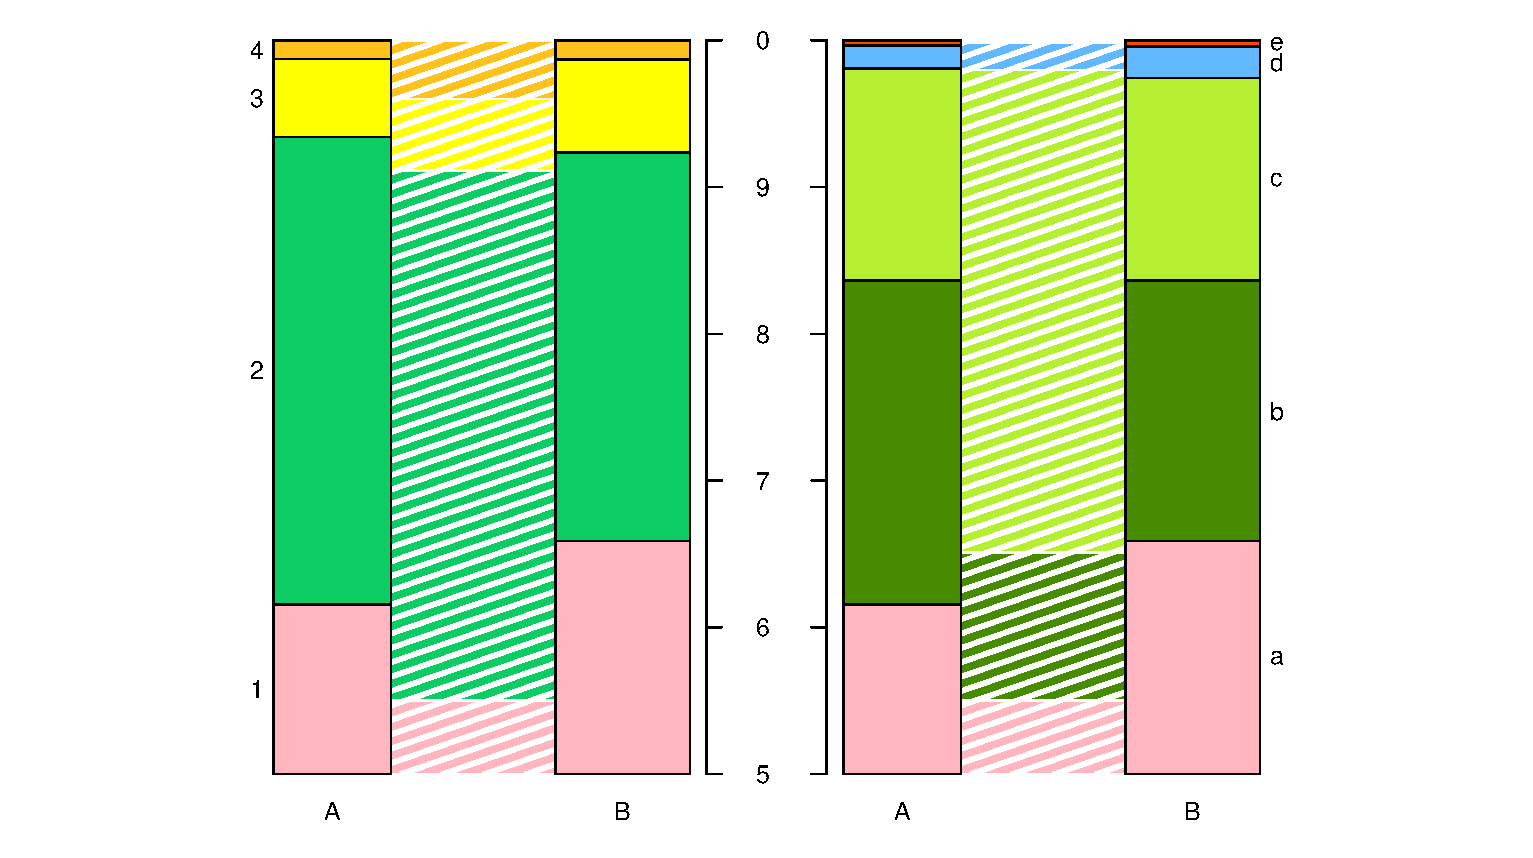
\includegraphics[width=7.425cm]{../figures/Ireland}}
\rput[bl](0.05,0.83) {\footnotesize Ireland (2011)\miniscule $N_{weighted} = 4,745,350$}
%\psframe(0,0)(1,1)
} 

\rput[bl](2.03,7.69){\large \textsc{Europe}
}

\rput[bl](2,5.66){
\psfrag{A}[c][b]{\miniscule{\begin{tabular}{@{}c@{}}
   \emph{Men}\\
   (10.58 \%)
\end{tabular}}}
\psfrag{B}[c][b]{\miniscule{\begin{tabular}{@{}c@{}}
   \emph{Women}\\
   (12.59 \%)
\end{tabular}}}
\rput[bl](0,0){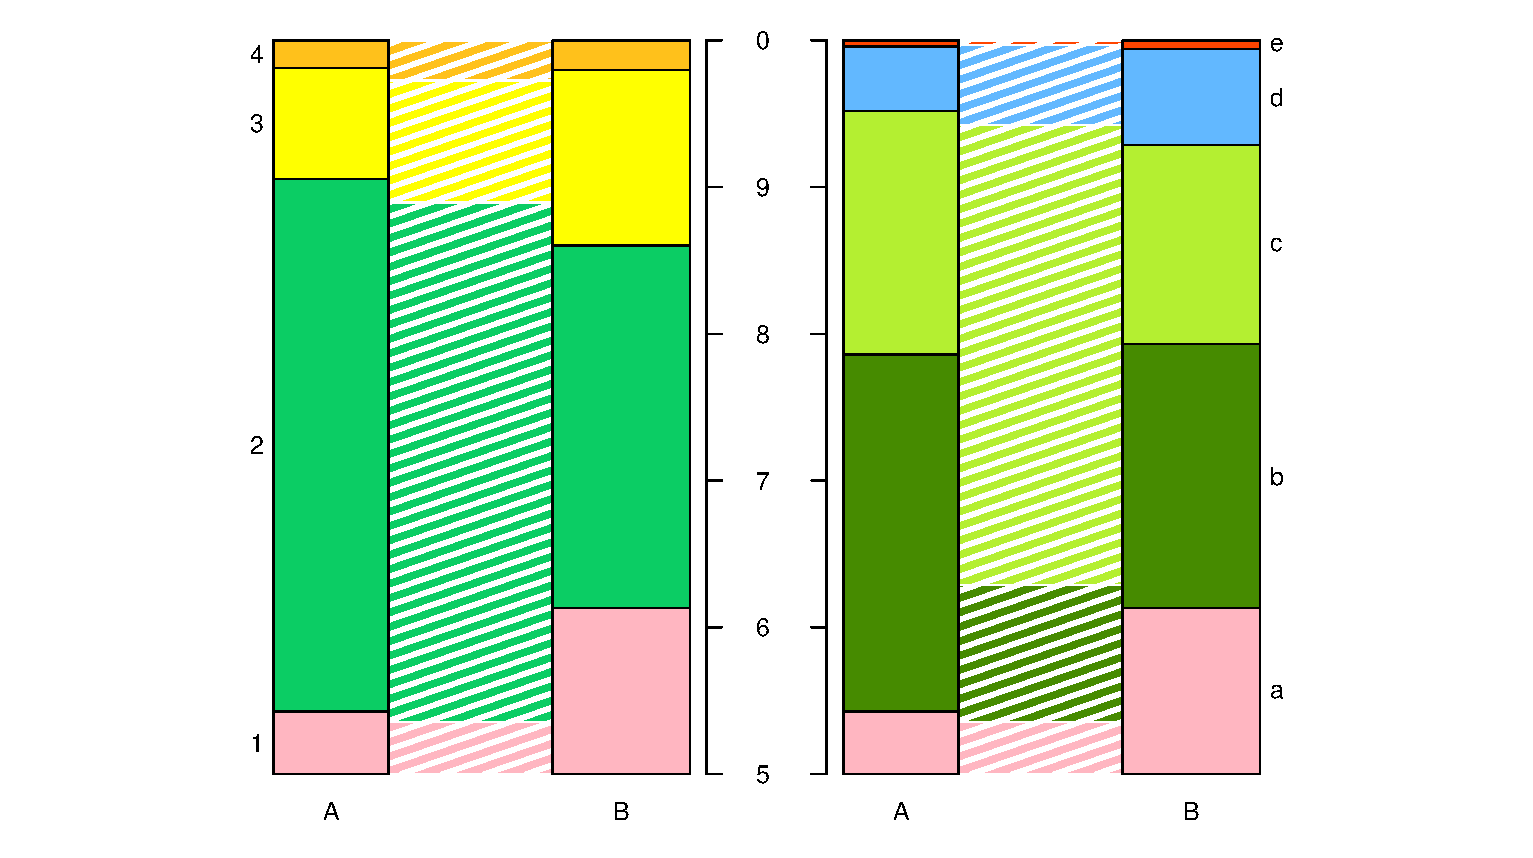
\includegraphics[width=7.425cm]{../figures/Greece}}
\rput[bl](0.05,0.83) {\footnotesize Greece (2001)\miniscule $N_{weighted} = 10,288,840$}
%\psframe(0,0)(1,1)
} 

\rput[bl](0.03,6.36){\large \textsc{Africa}
}
\rput[bl](0,5.33){
\psfrag{A}[c][b]{\miniscule{\begin{tabular}{@{}c@{}}
   \emph{Men}\\
   (2.88 \%)
\end{tabular}}}
\psfrag{B}[c][b]{\miniscule{\begin{tabular}{@{}c@{}}
   \emph{Women}\\
   (3.91 \%)
\end{tabular}}}
\rput[bl](0,0){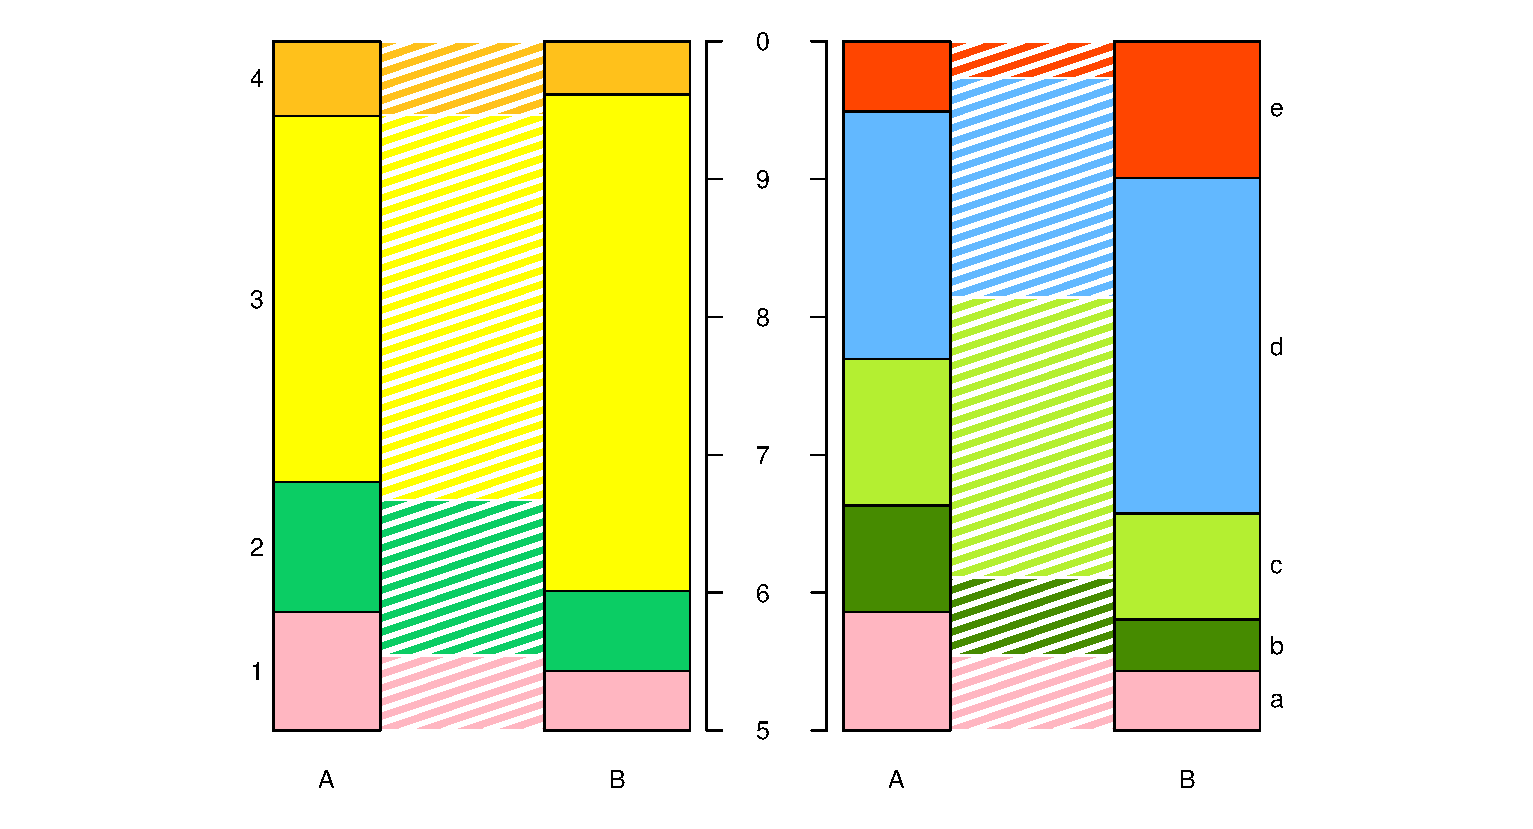
\includegraphics[width=7.425cm]{../figures/Botswana}}
\rput[bl](0.05,0.83) {\footnotesize Botswana (2011) \miniscule $N_{weighted} = 2,017,520$}
} 


\rput[bl](1,5.33){
\psfrag{A}[c][b]{\miniscule{\begin{tabular}{@{}c@{}}
   \emph{Men}\\
   (2.33 \%)
\end{tabular}}}
\psfrag{B}[c][b]{\miniscule{\begin{tabular}{@{}c@{}}
   \emph{Women}\\
   (3.68 \%)
\end{tabular}}}
\rput[bl](0,0){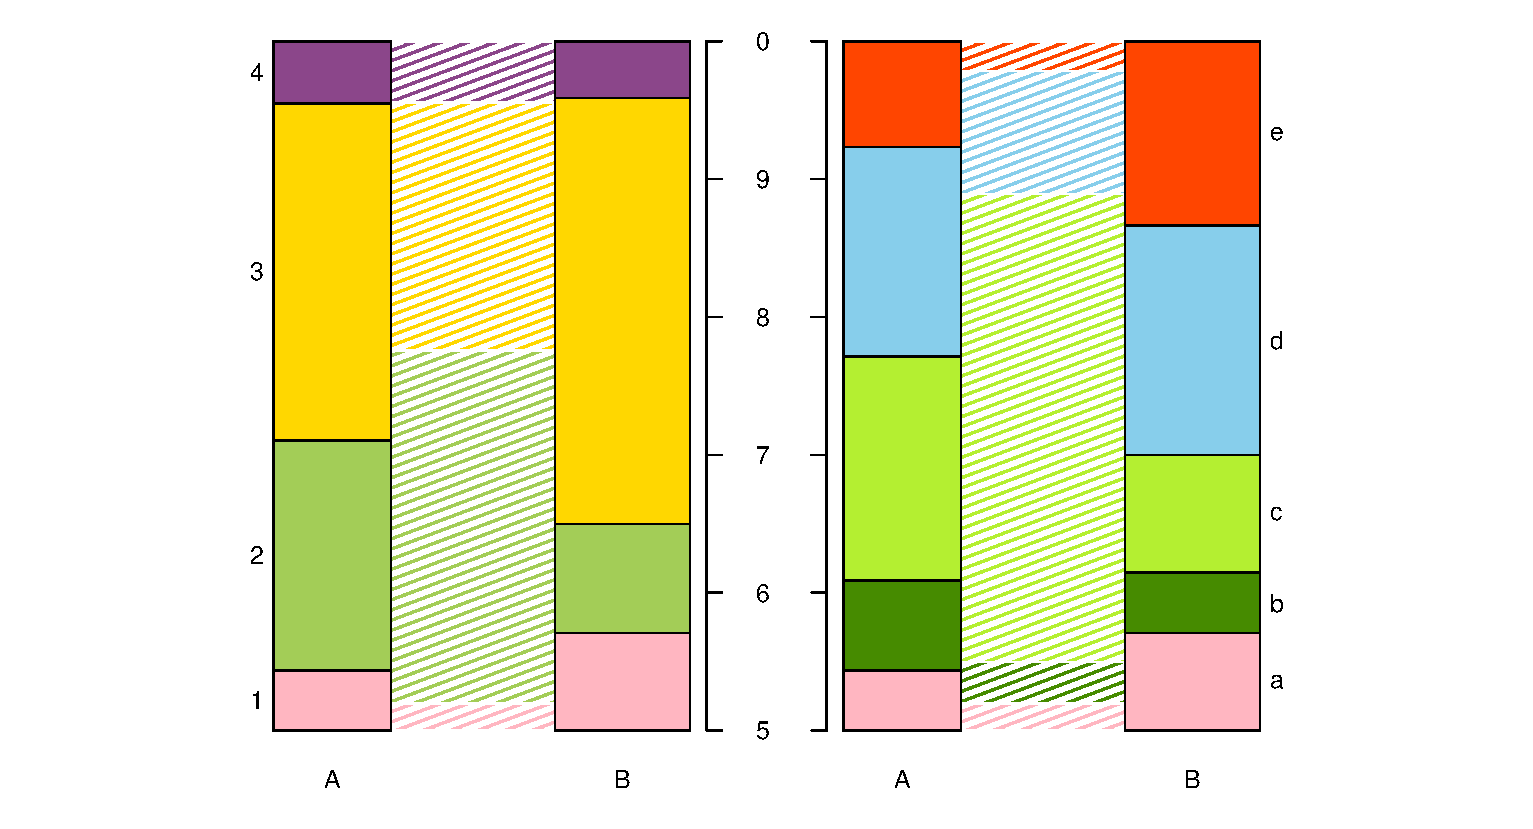
\includegraphics[width=7.425cm]{../figures/Kenya}}
\rput[bl](0.05,0.83) {\footnotesize Kenya (2009) \miniscule $N_{weighted} =  38,419,350$}
%\psframe(0,0)(1,1)
} 

\rput[bl](0,4.33){
\psfrag{A}[c][b]{\miniscule{\begin{tabular}{@{}c@{}}
   \emph{Men}\\
   (2.70 \%)
\end{tabular}}}
\psfrag{B}[c][b]{\miniscule{\begin{tabular}{@{}c@{}}
   \emph{Women}\\
   (2.71 \%)
\end{tabular}}}
\rput[bl](0,0){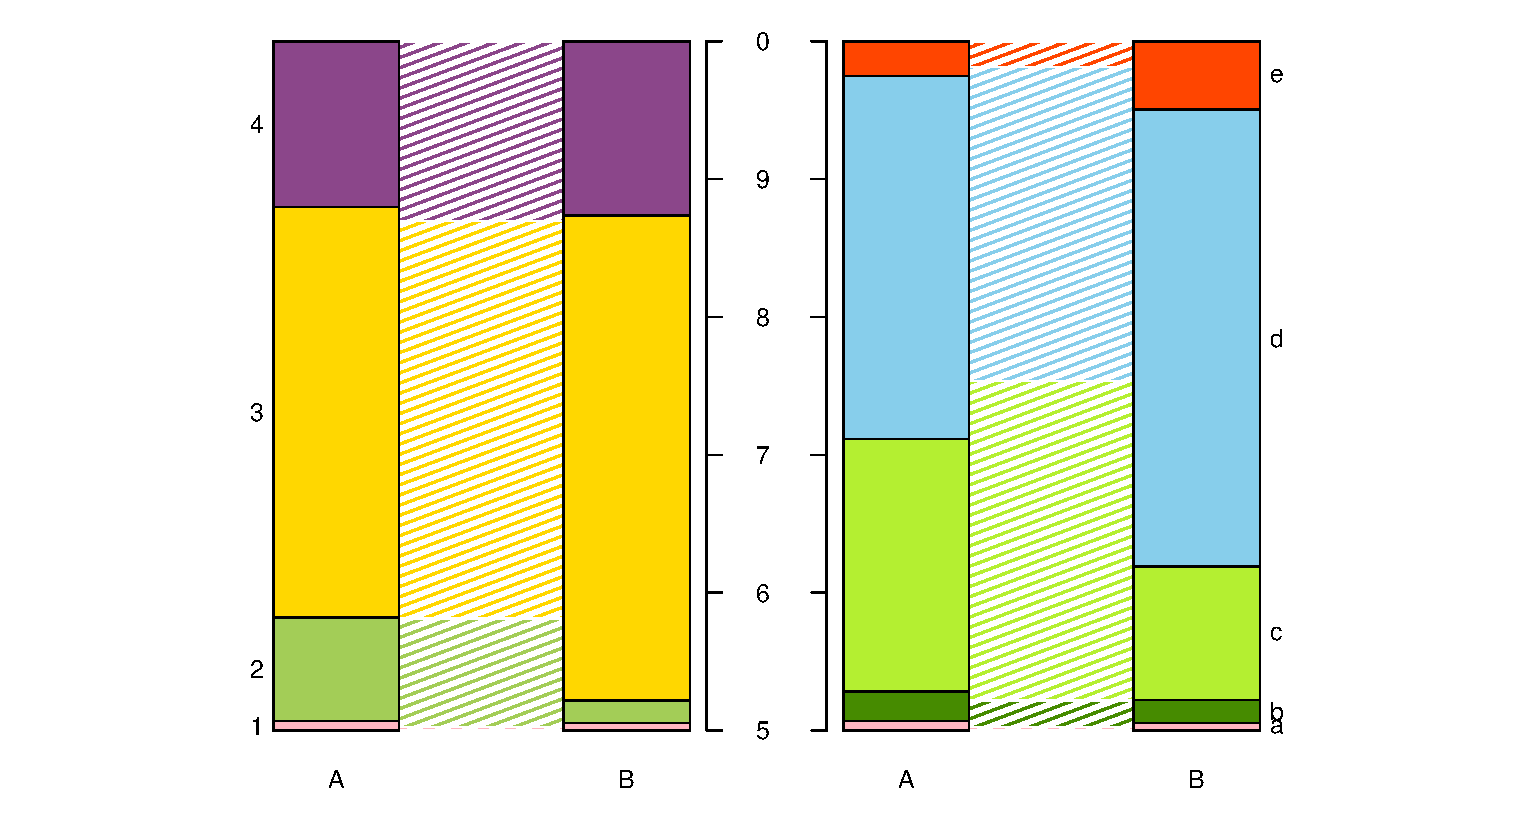
\includegraphics[width=7.425cm]{../figures/Senegal}}
\rput[bl](0.05,0.83) {\footnotesize Senegal (2002) \miniscule $N_{weighted} = 9,945,620$ }
%\psframe(0,0)(1,1)
} 

\rput[bl](1,4.33){
\psfrag{A}[c][b]{\miniscule{\begin{tabular}{@{}c@{}}
   \emph{Men}\\
   (3.18 \%)
\end{tabular}}}
\psfrag{B}[c][b]{\miniscule{\begin{tabular}{@{}c@{}}
   \emph{Women}\\
   (4.83 \%)
\end{tabular}}}
\rput[bl](0,0){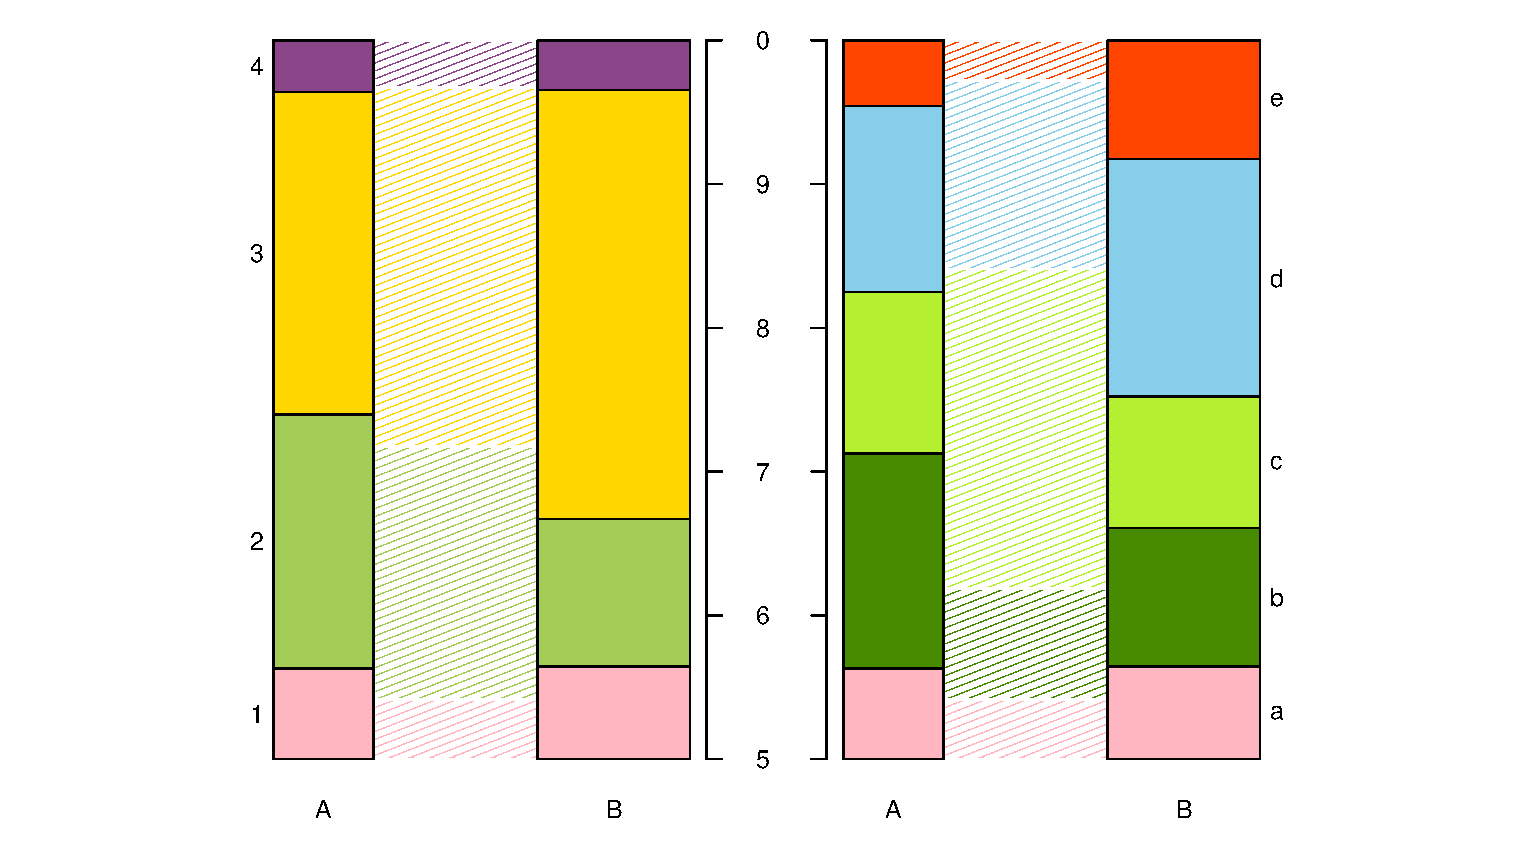
\includegraphics[width=7.425cm]{../figures/SouthAfrica}}
\rput[bl](0.05,0.83) {\footnotesize SouthAfrica(2011)\miniscule $N_{weighted} = 51,772,540$}
%\psframe(0,0)(1,1)
} 


}

\psset{xunit=1cm, yunit=1cm}

\rput[bl](22.3,1.3){
\rput[bl](0,0.2){
\mini{\parbox[c]
{6.6cm}{\scriptsize \textsc{References:}
\maxi \Urlmuskip=0mu plus 1mu\relax
\bibliographystyle{apa}
\renewcommand\refname{}
\vspace*{-2cm}
\minisculey{\bibliography{lit.bib}} 
}}}
}


\psset{xunit=1cm, yunit=1cm}
\psline[linewidth=0.5pt]{<->}(1,16.2)(1,17.2)
\end{pspicture}


\end{document}



